\documentclass[11pt]{article}
\usepackage{booktabs}
\usepackage{natbib}
\bibpunct[, ]{(}{)}{,}{a}{}{,}
\def\bibfont{\small}
\def\bibsep{\smallskipamount}
\def\bibhang{24pt}
\def\newblock{\ }
\def\BIBand{and}
\usepackage{latexsym,url,graphicx,amsmath,amssymb,setspace,amsfonts}
\usepackage{enumitem}
\usepackage{tgpagella}
\usepackage[dvipsnames]{xcolor}
\usepackage[most]{tcolorbox}
\tcbuselibrary{listings,breakable}
\usepackage[skip=8pt plus 1pt,indent=10pt]{parskip}
\usepackage[colorlinks,citecolor=hopkins-blue,urlcolor=hopkins-blue,linkcolor=hopkins-blue]{hyperref}
\usepackage{longtable}
\usepackage{booktabs}

\definecolor{hopkins-blue}{RGB}{0,45,114}
\definecolor{teal}{rgb}{0.0,0.5,0.5}

\newcommand{\edit}[1]{{\color{hopkins-blue}\itshape #1}}
\newcommand{\planned}{\noindent\underline{\textbf{Planned response}}:\ }
\newcommand{\expected}{\noindent\textbf{Expected outputs.} }

\setlength{\textwidth}{6.5in}
\setlength{\textheight}{8.8in}
\addtolength{\topmargin}{-\topmargin}
\setlength{\oddsidemargin}{0in}
\setlength{\evensidemargin}{0in}
\addtolength{\headsep}{-\headsep}
\addtolength{\topskip}{-\topskip}
\addtolength{\headheight}{-\headheight}
\allowdisplaybreaks
\sloppy


\usepackage{tcolorbox}
\definecolor{boxgrey}{RGB}{80,80,80}
\tcbuselibrary{breakable}


% WL response support: graph figures and fixed-placement result tables.
\usepackage{tikz}
\usetikzlibrary{arrows.meta,positioning}
\usepackage{float}
\definecolor{replyblue}{RGB}{0,65,165}
\definecolor{graphblue}{HTML}{0072B2}
\definecolor{graphgreen}{HTML}{009E73}
\definecolor{graphorange}{HTML}{D55E00}
\definecolor{graphgray}{HTML}{A6B1BA}
\tikzset{wlvariable/.style={circle,draw=graphgreen,fill=graphgreen!7,
 line width=.7pt,minimum size=7mm,inner sep=1pt,text=black,font=\small},
 row/.style={rectangle,rounded corners=1.5pt,draw=graphblue,fill=graphblue!7,
 line width=.7pt,minimum width=9mm,minimum height=6mm,inner sep=1pt,text=black,font=\small},
 added/.style={row,draw=graphorange,fill=graphorange!7},
 connection/.style={draw=graphgray,line width=.7pt},
 note/.style={text=black,font=\small,align=left}}
\newcommand{\WL}{\mathrm{WLsubtree}}
\newcommand{\toygraph}[7]{%
 \node[wlvariable] (#1v1) at (2.25,1.6) {#2};
 \node[wlvariable] (#1v2) at (2.25,0) {#3};
 \node[row] (#1r1) at (.25,1.6) {#4};
 \node[row] (#1r2) at (.25,0) {#5};
 \draw[connection] (#1r1)--(#1v1) (#1r1)--(#1v2)
                   (#1r2)--(#1v1) (#1r2)--(#1v2);
 \ifnum#6=1
  \node[added] (#1r3) at (.25,-.85) {#7};
  \draw[graphorange,line width=1pt] (#1r3)--(#1v1);
 \fi}

\begin{document}

\onehalfspacing

\begin{flushleft}
    \today \\
    Editors and the review team\\
    {\it Operations Research}\\
    \vspace{.6cm}
    Planned major revision of OPRE-2026-02-2704\\
    ``Large-Scale Optimization Model Auto-Formulation: Harnessing LLM Flexibility via Structured Workflow''\\
    \vspace{.6cm}
    Dear Editors and the review team,
\end{flushleft}

We thank the Associate Editor and both referees for their careful and constructive reports. We understand the central concern: the current numerical evidence is promising, but it does not yet establish the generalizability, robustness, scale, evaluation validity, and practical cost required to support the paper's broad claims. We agree that a major revision should be driven by stronger empirical evidence and a more precise statement of scope.

Below, we outline the experiments and revisions we plan to undertake, together with their expected outcomes.

Our revision will be organized around the following eight coordinated
changes:

\begin{enumerate}
    \item \textbf{Clarify and empirically isolate the distinguishing mechanism
    of LEAN-LLM-OPT.}
    We will retain LEAN-LLM-OPT as a multi-agent framework while positioning
    its central mechanism as category-conditioned, retrieval-augmented,
    knowledge-grounded procedural modeling. Ref-Data supplies non-parametric
    OR case knowledge, the category-conditioned scaffold specifies how this
    evidence should be used, and the formulation agent instantiates and
    executes the resulting task-specific modeling procedure using data tools.
    We will distinguish this mechanism from systems that maintain a persistent
    library of executable skills and add a controlled knowledge-by-procedure
    ablation that separately tests retrieved references, category conditioning,
    type-agnostic routing, and deliberately incorrect routing.

    \item \textbf{Strengthen the original benchmark through structural audit,
    controlled heterogeneity, provenance, and robustness tests.}
    We will freeze and retain the original 101 Large-Scale-OR instances for
    reproducibility, audit their problem types and structural archetypes, and
    acknowledge that several categories currently contain recurring canonical
    formulation patterns. We will then add paired parameter and structural
    variants for representative NRM, RA, TP, AP, and FLP instances. The
    structural variants will add or remove constraint families, modify
    objectives, or change variable, index, and interaction structures. We will
    complement these tests with instance-level provenance reporting and paired
    data-representation perturbations involving decoy rows, renamed or
    irrelevant columns, split datasets, and irrelevant files.

    \item \textbf{Directly evaluate reference dependence and generalization
    beyond closely matched cases.}
    We will compare Ref-Data and benchmark instances using both textual
    similarity and formulation-level structural similarity based on variables,
    objective terms, constraint families, index structures, and
    variable--constraint relationships. We will evaluate close references,
    distant same-category references, mismatched-category references, and
    no-reference conditions; remove the nearest references; and conduct
    leave-one-archetype-out and leave-one-type-out experiments. These analyses
    will show how formulation correctness changes as the target becomes less
    structurally similar to the available reference knowledge.

    \item \textbf{Replace optimal-value agreement with a richer formulation-
    correctness protocol.}
    Optimal-value matching will be retained only as a supplementary metric.
    The primary evaluation will use a blinded, equivalence-aware review in
    which anonymized formulations are independently assessed by at least two
    OR-trained evaluators, with disagreements resolved by a third evaluator.
    We will additionally report component-level correctness for variables,
    domains, parameter mappings, objective terms, and constraint families;
    evaluate generated solutions in the ground-truth formulation; measure
    feasibility violations and ground-truth optimality gaps; and perturb
    demands, capacities, inventories, and objective coefficients to expose
    missing or incorrect constraints that are nonbinding in the original
    instance.

    \item \textbf{Quantify classification dependence and evaluate a
    confidence-aware fallback.}
    We will report classification accuracy, macro-F1, per-type precision and
    recall, class confidence, and a confusion matrix. Downstream formulation
    correctness will be reported conditional on correct and incorrect routing.
    We will compare predicted routing with oracle routing, type-agnostic
    routing, and a true-type-by-routed-type sensitivity matrix obtained by
    deliberately sending instances through incorrect branches. For
    low-confidence instances, we will run the top-$k$ workflows and evaluate
    candidate formulations using prespecified ground-truth-free checks of query
    coverage, data mapping, structural consistency, model construction, and
    solver status. If no candidate can be selected reliably, the system will
    abstain and request clarification.

    \item \textbf{Improve baseline fairness, experimental transparency, and
    benchmark coverage.}
    We will add component-matched comparisons among LLM+Python/pandas,
    classification+retrieval+Python/pandas,
    classification+retrieval+FileQA/CSVQA without a type-tailored workflow,
    and the full LEAN-LLM-OPT pipeline. The primary comparison will use
    predicted routing, with oracle-routed counterparts used to quantify
    classification loss. All conditions will use the same base model, raw
    inputs, solver, decoding settings, timeout, and retry policy, and we will
    release the corresponding prompts, model versions, retrieval settings,
    tool definitions, and failure-handling procedures. We will present
    existing small-scale benchmarks as secondary evidence, add compatible
    ComplexOR and OptiBench instances, and reproduce OptiMUS on its native
    NLP4LP benchmark before presenting its Large-Scale-OR result as a separate
    cross-schema applicability test.

    \item \textbf{Separate input scale, formulation scale, runtime cost, and
    model-adaptation alternatives.}
    We will distinguish large input from large formulation and report input
    tokens, file and table dimensions, variables, constraints, and nonzero
    coefficients, including their minimum, quartiles, median, and maximum.
    Controlled scaling experiments for representative problem types will
    evaluate formulation correctness, solver time, and memory consumption. We
    will also report prompt and completion tokens, LLM and tool calls, latency,
    retries, and API cost for each pipeline stage and for all comparison
    methods. In addition, we will discuss how LEAN trajectories could support
    SFT, preference optimization, or RL distillation; compare their training,
    inference, and update costs with retrieval-based inference; and estimate
    the break-even query volume. If sufficient leakage-free training data are
    available, we will conduct a clearly labeled SFT pilot in which a smaller
    model replaces the formulation agent. We will not claim empirical benefits
    from full-pipeline RL without adequate leakage-free evidence.

    \item \textbf{Reframe and correct the Air-NRM case study.}
    We will consistently describe Air-NRM as a simulator-based case study
    rather than an operational deployment. We will distinguish the airline
    sales data used to train or calibrate the simulator from the simulated
    demand, booking, and optimization instances; provide complete definitions
    of all sets, indices, parameters, and variables; and make the
    exact-versus-at-most flight-cardinality requirement consistent across the
    query, formulation, implementation, and reported results. We will rerun
    affected experiments and clarify that the flow-balance constraint
    represents a long-run closed-loop flight-count balance rather than a full
    airline scheduling or fleet-routing model. The practical claims will be
    restricted accordingly.
\end{enumerate}


\begin{flushleft}
Warm regards,\\
The Authors
\end{flushleft}

%%%%%%%%%%%%%%%%%%%%%%%%%%%%%%%%%%%%%%%%%%%%%%%%%%%%%%%%%%%
\newpage
\begin{center}
{\LARGE\textbf{Response to Associate Editor}}
\end{center}

We thank you for recognizing the timeliness of the study and for identifying the two conceptual and empirical questions that should anchor the revision. We will use these questions to revise both the positioning of the framework and the design of the new robustness experiments.

\noindent\textbf{Comments:}

\begin{enumerate}[label=(AssoE.\arabic*),leftmargin=*]

\item \edit{The first one is about the positioning of the paradigm proposed in the paper. It seems to me that the main message of this paper is that it is important to have a ``reference'' for each class of problem rather than using a straightforward agent or fine-tuning approach. Using today's terminology, it would be useful to have a category-specific ``skill'' as well as ``knowledge'' to deal with domain specific questions. The authors may want to comment on this and perhaps connect with some advances in this area.}\label{asso-1}

We thank the Associate Editor for suggesting this perspective.
It helps clarify how LEAN-LLM-OPT combines reference modeling
knowledge with procedural guidance, and how this design relates
to recent work on agent skills.

Prior work distinguishes declarative knowledge---facts and
concepts relevant to a problem---from procedural
knowledge---strategies for carrying out a task
\citep{ae1_li2024metacognitive}. In LEAN-LLM-OPT, Ref-Data
primarily supplies declarative modeling knowledge through
reference problem descriptions, associated data, expert-provided
formulations, and annotations identifying relevant data.
These resources illustrate what a representative model contains
and how its data enter the formulation. Procedural guidance is
expressed through the modeling instructions, tool-use steps,
and output conventions that organize the use of these resources.
This is a distinction between their roles: a worked example
can also convey procedural information when presented as a
step-by-step demonstration.

This use of procedural guidance connects LEAN-LLM-OPT to agent
skills. \citet{ae1_zhou2026skillsurvey} describe skills as reusable
procedural artifacts organized around instructions, supporting
resources, and applicability conditions. Viewed through this
lens, LEAN-LLM-OPT's type-tailored modeling procedures are
\emph{skill-like}: classification identifies the applicable
route, modeling instructions specify how to proceed, and
reference cases supply supporting resources. The reusable
guidance is instantiated with a selected reference to construct
a demonstration, which the downstream agent adapts to the
target instance. Thus, reuse concerns the modeling method,
while the selected example and the subsequent reasoning and
tool use can vary across queries.

We distinguish this functional connection from specific
mechanisms for packaging and learning skills. SkillsBench
evaluates modular skill packages containing an instruction file
and optional supporting resources
\citep{ae1_li2026skillsbench}. Agent Workflow Memory induces
reusable workflows from task experience
\citep{ae1_wang2025awm}, while OptSkills distills optimization
trajectories into archetype-specific skills and supports their
refinement and expansion \citep{ae1_yang2026optskills}.
LEAN-LLM-OPT embeds procedural guidance in its workflow
construction and prompts; it does not maintain an independently
retrievable skill library or convert completed modeling
trajectories into new or revised skills. Its curated references
and reusable instructions remain fixed during evaluation.

Accordingly, LEAN-LLM-OPT remains an \emph{agentic workflow
construction framework} whose central mechanism is to organize
reference knowledge into procedural demonstrations for
optimization modeling with external data. LEAN-LLM-OPT connects knowledge and skills by organizing reference modeling knowledge into reusable, skill-like procedural guidance that agents adapt to the requirements and data of each problem.

We have added two discussions to the manuscript.
\emph{Knowledge and Skills in LLM Agents} in Section~1.2
(\emph{Related Works}) introduces the relevant terminology
and literature on knowledge, skill representation, and
skill learning. \emph{Connecting Reference Knowledge and
Modeling Skills} in Section~3.3
(\emph{Novelties in Our Design and Key Messages}) explains
how reference cases and procedural guidance work together
in LEAN-LLM-OPT, clarifies the roles of the workflow generation
and model generation agents, and distinguishes its skill-like
modeling procedures from a persistent skill library.

\item \edit{The second question concerns the heterogeneity of problems even within each category. In my opinion, the reason that the proposed method performed quite well may be attributed to the close resemblance between the reference problem and the actual problem. However, in reality, even when two problems belong to the same category, they can be still drastically different. For example, there could be many additional constraints, varying objectives, or other business requirements one may consider in one type of problem. Would the current approach be robust facing such conditions? How well can it perform? I didn't see clear evidence from the current paper. I hope that the authors can also perform some tests to analyze such scenarios.}\label{asso-2}

\begingroup\color{replyblue}
\textbf{Response.} We agree that a shared category does not establish a shared
formulation, and that the possibility of reference resemblance deserves a
direct examination. We therefore computed a Weisfeiler--Lehman (WL)
structural diagnostic for all 101 Large-Scale-OR benchmark formulations,
36 task variants, and the 15 LP files corresponding to the current
reference collection. To control for different ways of exporting variable
bounds, we analyze two consistently normalized representations and report
them separately: bounds retained in the \texttt{Bounds} section, and bounds
represented as explicit constraint rows. We also distinguish these
structural diagnostics from the complementary performance tests involving
task variants, leave-one-type-out (LOTO) evaluation, and forced routing.

\medskip
\textbf{Why a WL diagnostic is appropriate.}
The method combines two established components. Variable--constraint
bipartite graphs provide a natural way to represent MILP interactions
\citep{Gasse2019}. WL subtree kernels compare labeled graphs through
counts of progressively refined neighborhood patterns
\citep{Shervashidze2011}. Their combination allows us to compare explicit
formulation structure without relying on natural-language descriptions
or variable names.

Related MILP research learns graph-based instance similarities for
nearest-neighbor solver configuration \citep{Hosny2024}. That study
motivates comparing MILP instance representations, but uses a learned
metric related to solver costs. Here we choose an untrained WL feature
map so that every matched pattern and every calculation can be audited.
We use the literature to justify the representation and comparison
mechanism; it does not validate our scores as measures of business
semantics or solver performance.

The limitations are also grounded in MILP representation research.
\citet{Chen2023} show that their GNN class can fail to distinguish MILPs
with different feasibility properties. A recent arXiv manuscript by
\citet{Jahin2026}, whose record reports acceptance at TAG-DS 2026,
characterizes a class of MILP graph-transformer encoders as 1-WL bounded
under its stated input and architectural assumptions. These are
expressiveness results, not calibrations of a similarity threshold.
We accordingly use WL as a diagnostic of the selected labeled support
graph and retain these boundaries when interpreting the results.

\medskip
\textbf{Graph construction used in our implementation.}
We first apply the same bound-normalization rule to every reference,
benchmark instance, and variant. A linear row with exactly one nonzero
coefficient is converted to a bound: for example, $2x_j\leq6$ becomes
$x_j\leq3$, while a negative coefficient reverses the inequality.
Singleton equalities become coincident lower and upper bounds.
We intersect these restrictions with the native bounds, taking the
largest lower bound and the smallest upper bound. We then create two
representations:
\begin{enumerate}
\item \textbf{Bounds excluded from the graph.}
All effective bounds are stored in \texttt{Bounds}; their original
singleton rows are removed. Bounds still restrict the optimization
problem, but do not create graph nodes or edges. Finite bounds of integer
variables are represented by their ceiling/floor endpoints, preserving
the feasible integer lattice.
\item \textbf{Bounds included as constraint rows.}
Each effective finite lower and upper bound produces one explicit
inequality row. This includes default nonnegativity and binary $0/1$
bounds. Continuous and general integer variables are otherwise declared
free in \texttt{Bounds}; binary variables retain their intrinsic binary
domain. A fixed variable remains a variable node and has two coincident
bound rows. Duplicate or weaker singleton restrictions are not counted
again.
\end{enumerate}
Both representations retain variable domains, all remaining linear rows,
and all objectives. We do not perform general presolving, eliminate fixed
or isolated variables, or infer further bounds from multivariable rows.
Consequently, this normalization removes dependence on the storage
location and scaling of singleton bounds, but is not a complete
canonicalization of all mathematically equivalent formulations.

For formulation $P$, let $A_{aj}$ denote the coefficient of variable
$x_j$ in constraint row $a$ retained under the selected convention.
Following the original WL
notation, write its labeled graph as $G_P=(V,E,\ell)$, with
\[
 V=\mathcal V_{\rm var}\,\dot\cup\,\mathcal V_{\rm row},
 \qquad
 E=\big\{\{v_j,r_a\}:A_{aj}\ne0\big\}.
\]
Here $v_j$ and $r_a$ are variable and constraint nodes. We assign the
following initial labels:
\[
\ell(v_j)\in
\{\texttt{V:B},\texttt{V:I},\texttt{V:C}\},\qquad
\ell(r_a)=
\begin{cases}
 \texttt{R:E},&\text{equality},\\
 \texttt{R:I},&\text{inequality}.
\end{cases}
\]
Binary, integer, and continuous variables are therefore distinct.
Both $\leq$ and $\geq$ rows have label \texttt{R:I}.
The graph contains one edge per nonzero coefficient, with no coefficient
nodes or numerical edge attributes. Objectives, coefficient magnitudes
and signs, right-hand sides, bound values, and names are omitted.
The two conventions differ in whether effective bounds generate
inequality nodes and incident edges. We use the same labels and WL
calculation for both. The original WL paper defines a kernel on supplied
labeled graphs; it does not prescribe an optimization-specific choice
between these bound conventions.

\begin{figure}[ht]
\centering
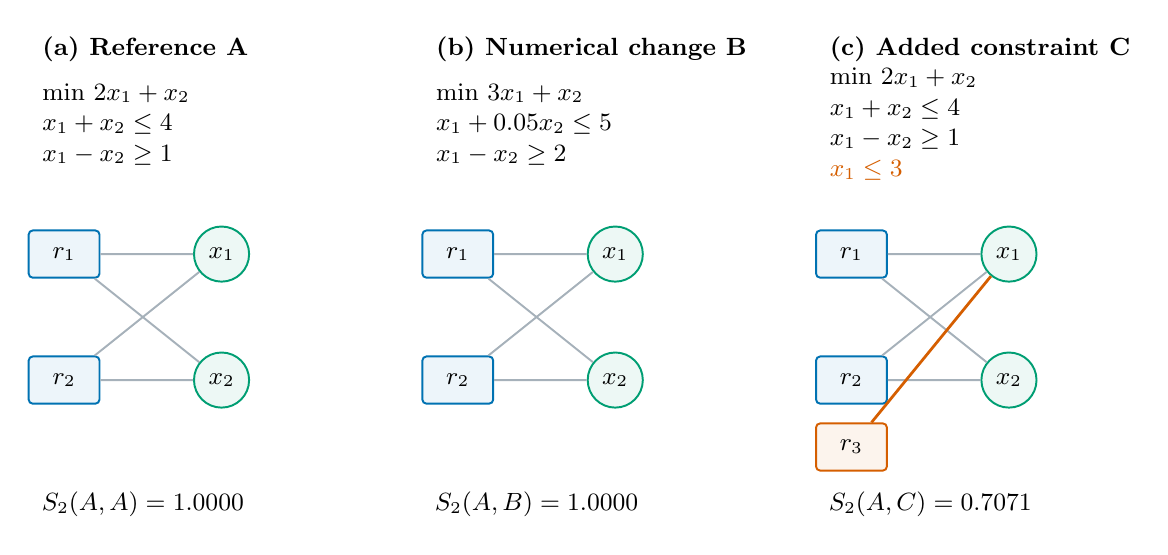
\begin{tikzpicture}[x=1cm,y=1cm]
 \begin{scope}[shift={(0,0)}]
  \node[note,anchor=west,font=\small\bfseries] at (-.15,4.2) {(a) Reference A};
  \node[note,anchor=west] at (-.15,3.25)
   {$\min\,2x_1+x_2$\\$x_1+x_2\leq4$\\$x_1-x_2\geq1$};
  \toygraph{a}{$x_1$}{$x_2$}{$r_1$}{$r_2$}{0}{}
  \node[note,anchor=north] at (1.25,-1.3) {$S_2(A,A)=1.0000$};
 \end{scope}
 \begin{scope}[shift={(5,0)}]
  \node[note,anchor=west,font=\small\bfseries] at (-.15,4.2) {(b) Numerical change B};
  \node[note,anchor=west] at (-.15,3.25)
   {$\min\,3x_1+x_2$\\$x_1+0.05x_2\leq5$\\$x_1-x_2\geq2$};
  \toygraph{b}{$x_1$}{$x_2$}{$r_1$}{$r_2$}{0}{}
  \node[note,anchor=north] at (1.25,-1.3) {$S_2(A,B)=1.0000$};
 \end{scope}
 \begin{scope}[shift={(10,0)}]
  \node[note,anchor=west,font=\small\bfseries] at (-.15,4.2) {(c) Added constraint C};
  \node[note,anchor=west] at (-.15,3.25)
   {$\min\,2x_1+x_2$\\$x_1+x_2\leq4$\\$x_1-x_2\geq1$\\
    \textcolor{graphorange}{$x_1\leq3$}};
  \toygraph{c}{$x_1$}{$x_2$}{$r_1$}{$r_2$}{1}{$r_3$}
  \node[note,anchor=north] at (1.25,-1.3) {$S_2(A,C)=0.7071$};
 \end{scope}
\end{tikzpicture}
\caption{Illustrative support graphs before the bound normalization used
for the two result tables. All variables are continuous and nonnegative (circle
nodes); all explicit rows are inequalities (rectangle nodes). Numerical
changes in B leave this graph unchanged. The additional explicit row in
C creates one node and one edge. For this teaching example only, the
common nonnegativity bounds are not drawn and $x_1\leq3$ remains an
explicit row. The score $0.7071$ therefore pertains to this illustrated
graph, not either fully normalized convention. Under bounds exclusion,
A and C instead have identical support graphs and similarity $1$.
These examples are not performance experiments.}
\label{fig:wl-encoding}
\end{figure}

\medskip
\textbf{WL refinement with the original paper's notation.}
We use the WL subtree kernel of Definition~4 in
\citet{Shervashidze2011}, with refinement as in Algorithms~1 and~2
and the input labels specified above. We compute the fixed-height
kernel through round $h$, without applying the early-stopping rule
of the isomorphism test.
Set $l_0(v)=\ell(v)$. At iteration $i\geq1$,
\[
 M_i(v)=\{\!\{l_{i-1}(u):u\in\mathcal N(v)\}\!\}.
\]
Here $\mathcal N(v)$ is the set of adjacent nodes, and double braces
denote a multiset: repeated neighbor labels are retained.
We form a signature by prefixing the sorted neighbor labels with the
node's own previous label:
\[
s_i(v)=\operatorname{concat}
\big(l_{i-1}(v),\operatorname{sort}(M_i(v))\big).
\]
Then
\[
 l_i(v)=f(s_i(v)),\qquad
 f(s_i(v))=f(s_i(w))\ \Longleftrightarrow\ s_i(v)=s_i(w).
\]
The injective dictionary implementing $f$ is shared across all 152 graphs
at each iteration, separately for each bound convention.
All nodes update synchronously from round $i-1$.
In code, a tuple stores the old label and sorted neighbor
labels; this is an unambiguous encoding of the same signature.
The compressed label identifiers are arbitrary; equal signatures receive
equal identifiers across graphs. At initialization, Algorithm~1 uses
$M_0(v):=l_0(v)=\ell(v)$; the neighbor-multiset formula applies only for
$i\geq1$. There is no $l_{-1}$ or refinement step at round zero.
Let $\Sigma_i=\{\sigma_{i1},\ldots,\sigma_{i|\Sigma_i|}\}$ be the shared
alphabet at iteration $i$, and let $c_i(G,\sigma)$ count occurrences of
label $\sigma$. The cumulative feature vector is
\[
\phi^{(h)}_{\WL}(G)=
\big(c_0(G,\sigma_{01}),\ldots,c_0(G,\sigma_{0|\Sigma_0|}),
\ldots,c_h(G,\sigma_{h1}),\ldots,c_h(G,\sigma_{h|\Sigma_h|})\big).
\]
We keep alphabets for different rounds disjoint by using
$(i,\text{label})$ as the feature key. The original subtree kernel is
\[
 k^{(h)}_{\WL}(G,G')=
 \langle\phi^{(h)}_{\WL}(G),\phi^{(h)}_{\WL}(G')\rangle
 =\sum_{i=0}^{h}\sum_{\sigma\in\Sigma_i}
 c_i(G,\sigma)c_i(G',\sigma).
\]
For reporting, we normalize this kernel:
\[
 S_h(P,Q)=
 \frac{k^{(h)}_{\WL}(G_P,G_Q)}
 {\sqrt{k^{(h)}_{\WL}(G_P,G_P)\,k^{(h)}_{\WL}(G_Q,G_Q)}}.
\]
This last normalization and the optimization-model labels are our
application choices; they are stated separately from the paper's
unnormalized kernel definition. Scores lie in $[0,1]$, with larger
values indicating closer normalized label-count vectors.

\begin{figure}[ht]
\centering
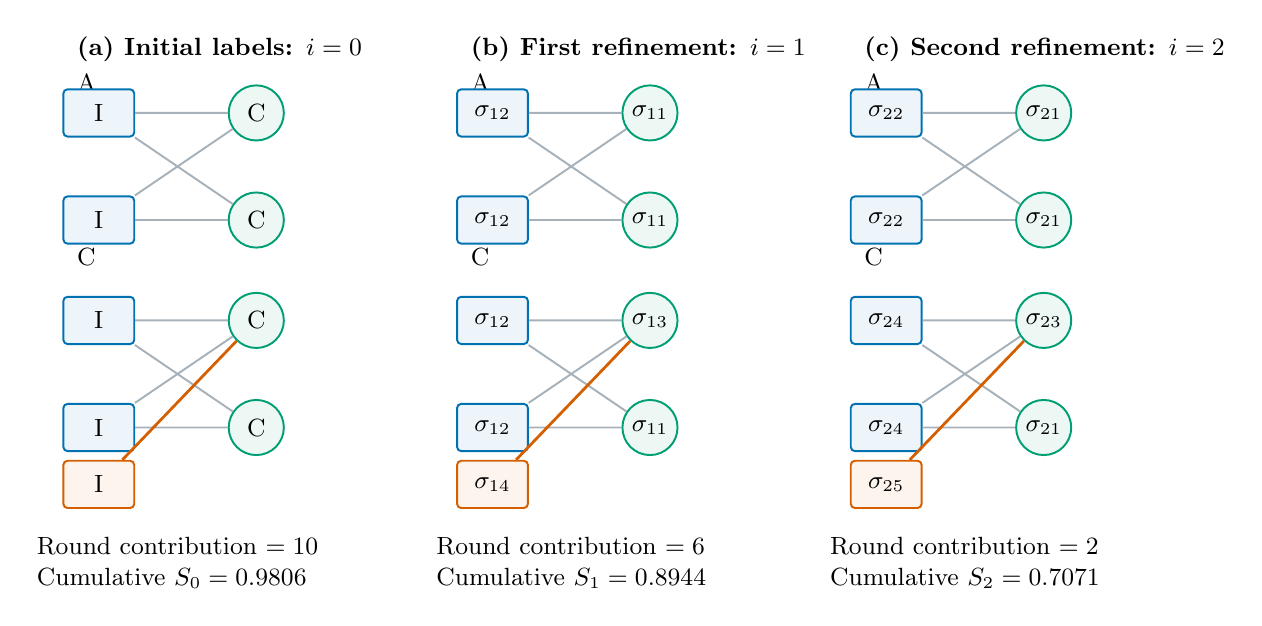
\begin{tikzpicture}[x=1cm,y=.85cm]
 \begin{scope}[shift={(0,0)}]
  \node[note,anchor=west,font=\small\bfseries] at (-.15,2.55) {(a) Initial labels: $i=0$};
  \node[note,anchor=west] at (-.15,2.05) {A};
  \toygraph{d}{C}{C}{I}{I}{0}{}
  \node[note,anchor=west] at (-.15,-.55) {C};
  \begin{scope}[shift={(0,-3.1)}]
   \toygraph{e}{C}{C}{I}{I}{1}{I}
  \end{scope}
  \node[note,anchor=north] at (1.25,-4.6)
   {Round contribution $=10$\\Cumulative $S_0=0.9806$};
 \end{scope}
 \begin{scope}[shift={(5,0)}]
  \node[note,anchor=west,font=\small\bfseries] at (-.15,2.55) {(b) First refinement: $i=1$};
  \node[note,anchor=west] at (-.15,2.05) {A};
  \toygraph{f}{$\sigma_{11}$}{$\sigma_{11}$}{$\sigma_{12}$}{$\sigma_{12}$}{0}{}
  \node[note,anchor=west] at (-.15,-.55) {C};
  \begin{scope}[shift={(0,-3.1)}]
   \toygraph{g}{$\sigma_{13}$}{$\sigma_{11}$}{$\sigma_{12}$}{$\sigma_{12}$}{1}{$\sigma_{14}$}
  \end{scope}
  \node[note,anchor=north] at (1.25,-4.6)
   {Round contribution $=6$\\Cumulative $S_1=0.8944$};
 \end{scope}
 \begin{scope}[shift={(10,0)}]
  \node[note,anchor=west,font=\small\bfseries] at (-.15,2.55) {(c) Second refinement: $i=2$};
  \node[note,anchor=west] at (-.15,2.05) {A};
  \toygraph{h}{$\sigma_{21}$}{$\sigma_{21}$}{$\sigma_{22}$}{$\sigma_{22}$}{0}{}
  \node[note,anchor=west] at (-.15,-.55) {C};
  \begin{scope}[shift={(0,-3.1)}]
   \toygraph{j}{$\sigma_{23}$}{$\sigma_{21}$}{$\sigma_{24}$}{$\sigma_{24}$}{1}{$\sigma_{25}$}
  \end{scope}
  \node[note,anchor=north] at (1.25,-4.6)
   {Round contribution $=2$\\Cumulative $S_2=0.7071$};
 \end{scope}
\end{tikzpicture}
\caption{WL propagation in the added-constraint example. C and I abbreviate
\texttt{V:C} and \texttt{R:I}; $\sigma_{ij}$ is the $j$th compressed label
at round $i$. Matching symbols within a round have matching signatures.
The new row first changes $x_1$'s label, then changes the labels of its
neighboring original rows. Round contributions are
$\sum_{\sigma\in\Sigma_i}c_i(G_A,\sigma)c_i(G_C,\sigma)$.
Scores use cumulative counts from rounds $0,\ldots,h$. As in
Figure~\ref{fig:wl-encoding}, this illustration leaves the added singleton
row explicit and does not normalize the common nonnegativity bounds.}
\label{fig:wl-rounds}
\end{figure}


\medskip
\textbf{Worked example: the A--C calculation.}
Write $\nu=\texttt{V:C}$ and $\rho=\texttt{R:I}$.
Superscripts identify the graph. In A, each variable is adjacent to
$r_1^A,r_2^A$, and each row is adjacent to $x_1^A,x_2^A$.
In C, $x_1^C$ is adjacent to all three rows, $x_2^C$ to the first two,
and $r_3^C$ only to $x_1^C$.

At round zero, variable labels are $\nu$ and row labels are $\rho$.
The count vectors in order $(\nu,\rho)$ are $(2,2)$ for A and
$(2,3)$ for C. The cross contribution is $10$, and their self
contributions are $8$ and $13$.

At round one, the following four groups cover every node.
The bracketed expression is the signature $s_1(v)$, formed from
the node's old label and its sorted neighbor multiset:
\[
\begin{aligned}
v\in\{x_1^A,x_2^A,x_2^C\}:&
\quad M_1(v)=\{\!\{\rho,\rho\}\!\},&
l_1(v)&=f(\langle\nu;\rho,\rho\rangle)=\sigma_{11},\\
v\in\{r_1^A,r_2^A,r_1^C,r_2^C\}:&
\quad M_1(v)=\{\!\{\nu,\nu\}\!\},&
l_1(v)&=f(\langle\rho;\nu,\nu\rangle)=\sigma_{12},\\
v=x_1^C:&
\quad M_1(v)=\{\!\{\rho,\rho,\rho\}\!\},&
l_1(v)&=f(\langle\nu;\rho,\rho,\rho\rangle)=\sigma_{13},\\
v=r_3^C:&
\quad M_1(v)=\{\!\{\nu\}\!\},&
l_1(v)&=f(\langle\rho;\nu\rangle)=\sigma_{14}.
\end{aligned}
\]
Thus the count vectors in alphabet order
$(\sigma_{11},\sigma_{12},\sigma_{13},\sigma_{14})$ are
$(2,2,0,0)$ and $(1,2,1,1)$.
The cross contribution is $2\cdot1+2\cdot2=6$;
self contributions are $8$ and $7$.

At round two, the five groups below again cover every node:
\[
\begin{aligned}
v\in\{x_1^A,x_2^A,x_2^C\}:&
\quad M_2(v)=\{\!\{\sigma_{12},\sigma_{12}\}\!\},\\[-2pt]
&\quad l_2(v)=f(\langle\sigma_{11};\sigma_{12},\sigma_{12}\rangle)
=\sigma_{21},\\
v\in\{r_1^A,r_2^A\}:&
\quad M_2(v)=\{\!\{\sigma_{11},\sigma_{11}\}\!\},\\[-2pt]
&\quad l_2(v)=f(\langle\sigma_{12};\sigma_{11},\sigma_{11}\rangle)
=\sigma_{22},\\
v=x_1^C:&
\quad M_2(v)=\{\!\{\sigma_{12},\sigma_{12},\sigma_{14}\}\!\},\\[-2pt]
&\quad l_2(v)=f(\langle\sigma_{13};
\sigma_{12},\sigma_{12},\sigma_{14}\rangle)=\sigma_{23},\\
v\in\{r_1^C,r_2^C\}:&
\quad M_2(v)=\{\!\{\sigma_{13},\sigma_{11}\}\!\},\\[-2pt]
&\quad l_2(v)=f(\langle\sigma_{12};\sigma_{11},\sigma_{13}\rangle)
=\sigma_{24},\\
v=r_3^C:&
\quad M_2(v)=\{\!\{\sigma_{13}\}\!\},\\[-2pt]
&\quad l_2(v)=f(\langle\sigma_{14};\sigma_{13}\rangle)=\sigma_{25}.
\end{aligned}
\]
The original rows in C see different round-one variable labels
$\sigma_{13},\sigma_{11}$; A's original rows see
$\sigma_{11},\sigma_{11}$. Hence their round-two labels differ.
However, $x_2^C$ still reads its neighbors' \emph{round-one}
labels, both $\sigma_{12}$, rather than their newly computed
round-two labels. It therefore matches A's variables.
Refinement adds no nodes or edges.

In alphabet order $(\sigma_{21},\ldots,\sigma_{25})$, the round-two
counts are $(2,2,0,0,0)$ and $(1,0,1,2,1)$.
Their cross contribution is $2$, and self contributions are $8,7$.
The cumulative feature vectors and similarities are
\[
\begin{aligned}
\phi^{(2)}_{\WL}(G_A)&=(2,2\,;\;2,2,0,0\,;\;2,2,0,0,0),\\
\phi^{(2)}_{\WL}(G_C)&=(2,3\,;\;1,2,1,1\,;\;1,0,1,2,1),\\
S_0(A,C)&=\frac{10}{\sqrt{8\cdot13}}=0.9806,\\
S_1(A,C)&=\frac{10+6}{\sqrt{(8+8)(13+7)}}=0.8944,\\
S_2(A,C)&=\frac{10+6+2}{\sqrt{(8+8+8)(13+7+7)}}=0.7071.
\end{aligned}
\]
Semicolons separate the rounds. The calculation uses all rounds up to
$h$, rather than just the last round, and was checked against the
benchmark WL module. Moving $x_1\leq3$ into excluded \texttt{Bounds}
makes A's and C's graphs identical, giving similarity $1$ despite
different feasible sets. Excluding bounds therefore does not
universally decrease similarity.

A score of $1$ means proportional feature vectors, not model equivalence.
For example, one eight-node alternating cycle and two disjoint
four-node alternating cycles have identical typed WL counts at every
depth despite different connectivity.

\medskip
\textbf{Reference matching and reproducibility.}
For a test formulation $P$ of category $g(P)$, let
$\mathcal R_{g(P)}$ denote its category's reference pool and
$\mathcal R$ the full collection. Within each bound convention,
\[
 S_{\rm same}(P)=\max_{R\in\mathcal R_{g(P)}}S_2(P,R),
 \qquad
 S_{\rm all}(P)=\max_{R\in\mathcal R}S_2(P,R).
\]
Nearest-reference matching means maximum similarity.
Each category's median and mean summarize these per-instance maxima;
the all-instance row pools individual scores, rather than averaging
category medians or means.
There is one reference each for NRM, RA, TP, AP, and UFLP, eight for
Mixture, and two for Others. Mixture matching does not merge Others.
Different candidate-pool sizes affect the maxima, and Others is a
heterogeneous pool rather than one modeling archetype.
All-reference scores concern the available collection, not necessarily
references retrieved during individual pipeline runs.
The 36 variants contain 3 AP, 3 UFLP, 17 Mixture, and 13 Others
instances; there are no NRM, RA, or TP variants in this set.

Both normalization procedures cover all 152 formulations.
Source LP and input CSV hashes remained unchanged.
Checks covered effective variable domains and bounds, retained rows,
objective sense and constants, and multiobjective metadata.
Each normalized model was exported to LP and MPS and read back.
Prior reconstruction of all 15 reference CSV Code fields verified
Code-to-LP correspondence; this does not independently certify every
natural-language modeling decision.
For explicit-bound conversion, 151 original/converted pairs returned
matching optimal objectives. The remaining pair, Other6, produced
feasible solutions with matching objectives within tolerance but did
not prove optimality within the time limit.
These checks concern conversion, not LLM accuracy.

We keep the existing primary depth $h=2$, report both bound conventions,
and do not choose settings to minimize similarity.
Symmetry, unit self-similarity, node-reordering invariance, and
disjoint-replication invariance were checked.
No learned classifier or fitted similarity threshold is used.

\begin{table}[H]
\centering\small\color{replyblue}
\caption{WL similarities with effective variable bounds stored in \texttt{Bounds} and excluded from the graph.}
\label{tab:ae-wl-bounds-excluded}
\setlength{\tabcolsep}{6pt}
\begin{tabular}{@{}lrrrr@{}}
\toprule
Category & Tests & Median $S_{\rm same}$ & Mean $S_{\rm same}$ &
Median $S_{\rm all}$\\
\midrule
\multicolumn{5}{@{}l}{\textbf{(a) Original Large-Scale-OR instances}}\\
NRM & 25 & 0.3234 & 0.3234 & 0.3330\\
RA & 22 & 0.6562 & 0.6564 & 0.6562\\
TP & 9 & 0.6240 & 0.6314 & 0.6343\\
AP & 5 & 0.0508 & 0.0551 & 0.4424\\
UFLP & 14 & 0.5503 & 0.5557 & 0.5503\\
Mixture & 18 & 0.3983 & 0.4499 & 0.5025\\
Others & 8 & 0.2584 & 0.3025 & 0.3811\\
\midrule
\textbf{All instances} & \textbf{101} & \textbf{0.5065} & \textbf{0.4632} & \textbf{0.5340}\\
\midrule
\multicolumn{5}{@{}l}{\textbf{(b) Task variants}}\\
NRM & 0 & --- & --- & ---\\
RA & 0 & --- & --- & ---\\
TP & 0 & --- & --- & ---\\
AP & 3 & 0.3569 & 0.3582 & 0.3569\\
UFLP & 3 & 0.1981 & 0.1972 & 0.3078\\
Mixture & 17 & 0.6665 & 0.6157 & 0.6665\\
Others & 13 & 0.2373 & 0.2993 & 0.4359\\
\midrule
\textbf{All instances} & \textbf{36} & \textbf{0.4325} & \textbf{0.4451} & \textbf{0.5588}\\
\bottomrule
\end{tabular}
\par\vspace{4pt}
\parbox{\linewidth}{\footnotesize
All values use cumulative rounds $0$--$2$ and cosine normalization;
higher means closer under this graph convention.
Each score first maximizes similarity over the specified reference pool.
All-instance rows pool the individual scores.
Dashes denote absent categories, not zero similarity.
Scores are not percentages of shared constraints or accuracy measures.}
\end{table}

\begin{table}[H]
\centering\small\color{replyblue}
\caption{WL similarities with effective finite variable bounds also represented as explicit constraint nodes.}
\label{tab:ae-wl-bounds-included}
\setlength{\tabcolsep}{6pt}
\begin{tabular}{@{}lrrrr@{}}
\toprule
Category & Tests & Median $S_{\rm same}$ & Mean $S_{\rm same}$ &
Median $S_{\rm all}$\\
\midrule
\multicolumn{5}{@{}l}{\textbf{(a) Original Large-Scale-OR instances}}\\
NRM & 25 & 0.6097 & 0.6097 & 0.8494\\
RA & 22 & 0.8335 & 0.8210 & 0.8335\\
TP & 9 & 0.8245 & 0.8275 & 0.8293\\
AP & 5 & 0.2169 & 0.2166 & 0.6146\\
UFLP & 14 & 0.7740 & 0.7735 & 0.7740\\
Mixture & 18 & 0.6779 & 0.6993 & 0.7723\\
Others & 8 & 0.6477 & 0.6060 & 0.6790\\
\midrule
\textbf{All instances} & \textbf{101} & \textbf{0.7271} & \textbf{0.6940} & \textbf{0.8335}\\
\midrule
\multicolumn{5}{@{}l}{\textbf{(b) Task variants}}\\
NRM & 0 & --- & --- & ---\\
RA & 0 & --- & --- & ---\\
TP & 0 & --- & --- & ---\\
AP & 3 & 0.6079 & 0.6074 & 0.6109\\
UFLP & 3 & 0.5615 & 0.5608 & 0.6346\\
Mixture & 17 & 0.8340 & 0.8141 & 0.8340\\
Others & 13 & 0.6174 & 0.6107 & 0.7157\\
\midrule
\textbf{All instances} & \textbf{36} & \textbf{0.6793} & \textbf{0.7023} & \textbf{0.7676}\\
\bottomrule
\end{tabular}
\par\vspace{4pt}
\parbox{\linewidth}{\footnotesize
All values use cumulative rounds $0$--$2$ and cosine normalization;
higher means closer under this graph convention.
Each score first maximizes similarity over the specified reference pool.
All-instance rows pool the individual scores.
Dashes denote absent categories, not zero similarity.
Scores are not percentages of shared constraints or accuracy measures.}
\end{table}


\medskip
\textbf{Results and interpretation.}
With bounds retained only in \texttt{Bounds}
(Table~\ref{tab:ae-wl-bounds-excluded}), the 101-instance same-category
median is $0.5065$, its mean is $0.4632$, and the all-reference median
is $0.5340$. With bounds also represented as constraint rows
(Table~\ref{tab:ae-wl-bounds-included}), the corresponding values are
$0.7271$, $0.6940$, and $0.8335$.
Resemblance therefore varies by category and by the information
included in the graph.

RA's same-category median changes from $0.6562$ to $0.8335$,
TP's from $0.6240$ to $0.8245$, and UFLP's from $0.5503$ to
$0.7740$ when bounds are included.
Common bound rows add similarly labeled leaf nodes and alter the
refinement signatures of neighboring variables.
They increase category medians on these data, although the A--C
example demonstrates that this direction is not universal.
Changing the storage location of a bound does not change the
mathematical problem: the diagnostics measure different selected
representations.

Allowing any reference also reveals resemblance missed by
same-category matching. AP's median rises from $0.0508$ to $0.4424$
under bounds exclusion, and from $0.2169$ to $0.6146$ under bounds
inclusion. Mixture's corresponding values rise from $0.3983$ to
$0.5025$, and from $0.6779$ to $0.7723$.
A difference from the designated category template is therefore
not a difference from every available reference.

The variant same-category median is $0.4325$ under bounds exclusion
and $0.6793$ under inclusion; all-reference medians are $0.5588$
and $0.7676$. Under exclusion, category medians range from $0.1981$
for UFLP to $0.6665$ for Mixture.
Because the original and variant sets have different category
compositions, their pooled medians do not establish that every
variant is less similar, more complex, or farther from its own original.

Three qualifications are especially relevant to the AE's concern.
\begin{enumerate}
\item \textbf{NRM reflects a reference revision.}
All singleton restrictions in the 25 NRM tests become bounds.
Under exclusion, their graphs retain integer variable nodes but
have no row nodes or edges.
The current NRM reference contains a synthetic shared-dispatch row
coupling four variables, added in an earlier revision after
inspecting reference resemblance. This largely explains the score
$0.3234$. Removing only this row from a separate diagnostic copy
restores all 25 scores to $1$ under either normalized convention.
The lower NRM scores describe the revised reference; they do not
independently establish test heterogeneity or robustness to new
test-side requirements.

\item \textbf{AP includes a variable-domain difference.}
The five original AP exports use continuous variables, whereas their
reference uses binary variables. This changes the initial labels
and subsequent refinements. The low score does not by itself
establish different business requirements.
Under standard assignment assumptions, a continuous relaxation can
have integral optimal solutions; its graph encoding still differs here.

\item \textbf{WL is not a calibrated novelty test.}
No universal high/low threshold is assumed.
A score of $0.5065$ is not $50.65\%$ shared constraints or business rules.
One original UFLP instance attains similarity $1$ under both
conventions, so overlap remains present.
The $h=1,2,3$ pooled same-category medians are
$0.6748,0.5065,0.4005$ with bounds excluded and
$0.9007,0.7271,0.5782$ with bounds included.
We retain $h=2$ without selecting depth to lower the score.
\end{enumerate}

The diagnostics quantify local structural differences and shared
patterns, partially addressing the possibility that category labels
or semantic comparisons conceal formulation overlap.
They do not rule out shared templates or prove generalization to
unseen archetypes. Objectives, coefficient values and signs, and
right-hand-side changes are outside this encoding.

\medskip
\textbf{Complementary performance evidence for robustness.}
To address performance, we also evaluated task variants, LOTO
reference withholding, and forced routing.
These interventions change the task or its available modeling
support; WL itself only measures formulation resemblance.

The saved 36-variant evaluation completed 30 of 36 instances and
matched the reference objective on 29 of 36 ($80.56\%$).
In the saved GPT-4.1 LOTO examples-and-route experiment,
matching category examples were removed and the corresponding
execution route disabled. The pipeline completed 94 of 101
instances and matched the objective on 88 of 101 ($87.13\%$),
compared with 95 of 101 ($94.06\%$) for that experiment's saved
full baseline, a decrease of $6.93$ percentage points.
This evaluates a specified withholding intervention, not complete
removal of all prior knowledge about the category.

The saved forced-routing evaluation applies six execution routes
to each of the 101 problems.
Among the 505 assignments to a route different from the designated
route, 474 returned a solution and 431 matched the reference
objective ($85.35\%$ of all 505 assignments).
These are repeated assignments to 101 problems, not 505 independent
benchmark problems. Forced routing fixes an execution route;
route withholding instead lets the classifier choose among the
remaining routes. The interventions are distinct.

All objective-match rates use relative and absolute tolerances
$10^{-4}$, with failures included in the denominator.
Objective matching is a performance indicator, not proof that every
constraint and modeling decision is correct.
The variant, LOTO, and forced-routing records come from their
respective saved implementation snapshots; their rates should not
be pooled or treated as a common-version head-to-head comparison.
The bound-normalization analysis did not rerun LLM evaluations.

Together, these structural diagnostics and performance experiments
provide complementary evidence of resilience within the evaluated
settings, while exposing remaining failures.
We therefore qualify the robustness claim: the evidence supports
performance beyond reliance on a single intact same-category
reference template, but does not establish universal robustness
to arbitrary new constraints, objectives, or business requirements.
\endgroup

\end{enumerate}

\newpage
\begin{center}
{\LARGE\textbf{Response to Reviewer 1}}
\end{center}

We thank you for evaluating the paper according to the rigor and generalizability of its empirical evidence. We agree that these are the appropriate standards for the contribution. Below, we restate each major comment in italic font and describe the evidence we plan to add.

\noindent\textbf{Major Comments:}

\begin{enumerate}[label=(R1.Major.\arabic*),leftmargin=*]

\item \edit{At present, I am not fully convinced that the evidence establishes generalizable performance. The main benchmark, Large-Scale-OR, is author-constructed from Kaggle-style datasets, expert-generated labels, and imputed parameters; the Air-NRM case is based on simulated airline datasets rather than a documented operational deployment. The paper provides semantic similarity comparisons between Ref-Data and the benchmarks, but it does not rule out structural overlap or benchmark-construction choices that favor the proposed type-tailored workflow.

The authors should strengthen the empirical validation by clearly reporting which data and parameters are real, synthetic, imputed, or simulated. Besides, the current benchmark demonstrates performance on the authors' constructed distribution of problem types and data schemas. It does not yet establish robustness to realistic perturbations in data representation, irrelevant records, or unseen modeling archetypes. Since the paper's contribution is primarily empirical, and the authors motivate this study by claiming that large-scale inputs are heterogeneous, I would like to see controlled robustness tests such as decoy-row insertion, renamed/irrelevant columns, split datasets, and leave-one-type-out evaluation.}\label{R1-major-1}



%\planned We will strengthen the evaluation in four ways.

%First, we will add an instance-level provenance table. For every query, dataset, parameter, label, and ground-truth formulation, we will record whether it comes from a public or industry source, a simulator, a synthetic generator, an imputation rule, or expert authoring. For Air-NRM, we will clearly distinguish the real sales data used to calibrate the simulator from the downstream simulated data and labels. We will also state explicitly that Air-NRM is a simulator-based case study and not an operational deployment.

%Second, we will create controlled variants of the existing instances while keeping the underlying optimization problem and ground-truth formulation unchanged. These tests will include decoy-row insertion, renamed or irrelevant columns, splitting one dataset into multiple files, and irrelevant files. We will evaluate each perturbation separately and in combination, and compare the result with the corresponding unmodified instance. This will show whether the system can identify the relevant data rather than relying on a fixed schema or a particular file organization.

%Third, we will evaluate generalization to unseen modeling types. In a leave-one-type-out experiment, we will remove all Ref-Data instances from one problem type and test the system on that type. We will repeat this procedure for each type and report both formulation correctness and the failure rate. This will distinguish performance obtained from adapting a known type from performance on a type for which no reference case is available.

%Finally, we will compare Ref-Data and benchmark instances using both textual and formulation-level structural similarity. The structural comparison will consider variables, objective terms, constraint families, index structures, and variable--constraint relationships. For each test instance, we will report the similarity and distance to its nearest reference cases, identify possible exact or near-duplicate formulations, and analyze performance across close, medium-distance, and distant reference groups. We will also repeat the evaluation after removing closely related references.

%All experiments will use the same prompts, model settings, retrieval budget, and evaluation protocol across methods. We will report formulation and component-level correctness, feasibility violations, objective gaps, and performance changes relative to the unperturbed instances. These results will allow us to separate improvements due to the LEAN workflow from improvements that may arise from benchmark construction or close structural matches in Ref-Data.

%\expected An instance-level provenance table; paired data-perturbation experiments; leave-one-type-out results; textual and formulation-level similarity analyses between Ref-Data and the benchmarks; nearest-reference and reference-removal results; and revised generalization claims based on the observed robustness and structural-overlap evidence.

\noindent\textbf{Response:(jm)}

We thank the reviewer for this important comment. We agree that the generalizability of the empirical evidence should be examined from several complementary perspectives. We address the reviewer's concerns in four
parts below.

\vspace{2mm}
\noindent\textbf{1. Data and Parameter Provenance}

% ========================================================
% Response to be added:
% - Distinguish observed, transformed, imputed, and
%   synthetic data/parameters.
% - Refer to the newly added ``Data Provenance and
%   Instance Construction'' subsection.
% - Explain parameter-level provenance for the five base
%   problem classes and for Others/Mixture.
% ========================================================

We agree that the previous manuscript did not sufficiently distinguish the
provenance of the source data and the optimization-specific parameters used
to construct Large-Scale-OR. To improve this transparency, we added a new
subsection, ``Data Provenance and Instance Construction,'' which describes
how the source data are converted into the parameters used in the final
optimization instances.

We now distinguish four parameter-level provenance categories:
\textit{Observed}, \textit{Transformed}, \textit{Imputed}, and
\textit{Synthetic}. Observed parameters retain values directly from the
source dataset; Transformed parameters are deterministically derived from
observed values; Imputed parameters are constructed using predefined rules
when optimization-specific inputs are unavailable in the source data; and
Synthetic parameters are generated according to predefined distributions or
canonical optimization formulations. This distinction allows us to describe
the provenance of individual optimization parameters rather than assigning a
single ``real'' or ``synthetic'' label to an entire instance.

For the five canonical problem classes (NRM, TP, FLP, RA, and AP), we now
report the mapping from source fields to final optimization parameters,
together with their provenance and construction procedures. For example, the
new provenance table for NRM is reproduced below:

\begin{center}
\small
\setlength{\tabcolsep}{6pt}
\renewcommand{\arraystretch}{1.12}
\begin{tabular}{lll}
\hline
\textbf{Final Parameter}
& \textbf{Source Field}
& \textbf{Provenance} \\
\hline
Product Name
& Product id
& Observed \\

Revenue
& Unit selling Price
& Transformed \\

Demand
& Units sold
& Imputed \\

Initial Inventory
& Units sold
& Imputed \\
\hline
\end{tabular}
\end{center}

As shown in the table, the product identifier is retained directly from the
source data, while revenue is transformed from the observed selling price.
Demand and initial inventory are not directly available as optimization
parameters and are therefore imputed from historical units sold using the
predefined construction rules reported in the revised appendix. We provide
the same parameter-level provenance description for TP, FLP, RA, and AP.
For AP, where no suitable source dataset directly provides the required
worker--task cost matrix, the worker set, task set, and assignment costs are
classified as Synthetic. Because instances within these canonical classes
follow standardized construction procedures, we report these mappings at the
problem-class level rather than repeating the same construction rules for
individual instances.

We separately describe the construction of the heterogeneous Others and
Mixture categories, which do not share a common parameter schema. Others
contains established optimization archetypes outside the five primary
classes, including problems drawn from real-world applications, textbook
exercises, and representative formulations reported in the literature.
Mixture instances are primarily constructed by combining, extending, or
modifying the base problem classes, with inherited parameters following the
corresponding provenance treatment and additional parameters introduced
according to the requirements of the extended formulation. In the
representative Mixture instance reported in the appendix, for example,
product identifiers and base product profits are retained from the source
retail data, whereas labor and material requirements and resource capacities
are generated synthetically.

With these additions, the reader can now see more directly which inputs come
from the source data and which are introduced during benchmark construction,
as well as the rules used to construct the latter. We next examine whether
the results are robust to these construction choices and to changes in how
the input data are represented.

\vspace{2mm}
\noindent\textbf{2. Robustness to Benchmark Construction and Data Representation}

% ========================================================
% Response to be added:
% - Address the concern that benchmark-construction
%   choices may favor the proposed type-tailored workflow.
% - Report robustness to structural variants.
% - Report robustness to changes in data representation,
%   including renamed/irrelevant columns, decoy rows,
%   split datasets, and irrelevant files.
% ========================================================

[Response to be added.]

\vspace{2mm}
\noindent\textbf{3. Leave-One-Type (LOTO) Evaluation}

To examine the dependence on type-specific reference examples and workflow availability, we conducted two complementary test-time leave-one-type-out (LOTO) evaluations on Large-Scale-OR using GPT-4.1.

Both experiments use seven folds defined by the annotated problem types: TP, NRM, RA, FLP, AP, Mixture, and Others. Each fold evaluates the problems belonging to its held-out type, giving 101 distinct problems per experiment. Classification is performed again under the corresponding fold's conditions. We distinguish successful execution from agreement with the reference objective value. Objective agreement uses the original absolute and relative tolerances of \(10^{-4}\); execution failures remain in the denominator of the overall objective-match rate.

\medskip
\noindent\textbf{Experiment 1: withholding same-type reference examples}

For each held-out type, we removed all entries carrying that semantic label from the external example library used for retrieval. Classification, formulation, and code-generation components used the filtered library wherever they accessed these examples. All workflow routes remained available, including the route corresponding to the held-out type. Mixture and Others entries were removed separately, although their labels share the Others workflow; therefore, examples from the other semantic category could remain available to that shared workflow.

The following classification matrix shows the number of problems assigned to each predicted label. Rows represent the annotated held-out type and columns represent the predicted semantic label. These counts include problems whose subsequent execution failed.

\begin{center}
\small
\setlength{\tabcolsep}{5pt}
\renewcommand{\arraystretch}{1.12}
\begin{tabular}{lrrrrrrr}
\hline
\shortstack[l]{Held-out\\type}
& TP & NRM & RA & FLP & AP & Mixture & Others \\
\hline
TP      & 9 & 0  & 0  & 0  & 0 & 0  & 0 \\
NRM     & 0 & 23 & 2  & 0  & 0 & 0  & 0 \\
RA      & 0 & 0  & 22 & 0  & 0 & 0  & 0 \\
FLP     & 0 & 0  & 0  & 14 & 0 & 0  & 0 \\
AP      & 0 & 0  & 0  & 0  & 5 & 0  & 0 \\
Mixture & 0 & 0  & 4  & 0  & 0 & 12 & 2 \\
Others  & 0 & 0  & 1  & 0  & 0 & 0  & 7 \\
\hline
\end{tabular}
\end{center}

The classifier correctly labelled \textbf{92/101 problems (91.09\%)}. Specifically, two NRM problems were assigned to RA; four Mixture problems were assigned to RA and two to Others; and one Others problem was assigned to RA. Predicted Mixture and Others labels both invoke the Others route; all other labels invoke their correspondingly named routes.

The execution and objective-match results for this experiment are reported separately below.

\begin{center}
\small
\setlength{\tabcolsep}{5pt}
\renewcommand{\arraystretch}{1.12}
\begin{tabular}{lrrrrr}
\hline
\shortstack[l]{Held-out\\type}
& Cases
& Solved
& \shortstack{Objective\\matches}
& \shortstack{Solve\\rate (\%)}
& \shortstack{Objective-match\\rate (\%)} \\
\hline
TP      & 9  & 6  & 5  & 66.67  & 55.56 \\
NRM     & 25 & 14 & 14 & 56.00  & 56.00 \\
RA      & 22 & 10 & 10 & 45.45  & 45.45 \\
FLP     & 14 & 12 & 12 & 85.71  & 85.71 \\
AP      & 5  & 5  & 5  & 100.00 & 100.00 \\
Mixture & 18 & 15 & 15 & 83.33  & 83.33 \\
Others  & 8  & 8  & 7  & 100.00 & 87.50 \\
\hline
\textbf{Total}
& \textbf{101}
& \textbf{70}
& \textbf{68}
& \textbf{69.31}
& \textbf{67.33} \\
\hline
\end{tabular}
\end{center}

Overall, \textbf{70/101 problems (69.31\%)} completed execution successfully, and \textbf{68/101 (67.33\%)} matched the reference objective. The remaining outcomes comprised 31 execution failures and two successfully executed cases with non-matching objectives. These results provide evidence that correct classification and reference-matching results remain possible after removing same-labelled retrieved examples, while also showing that this intervention does not eliminate execution failures or objective mismatches.

\medskip
\noindent\textbf{Experiment 2: withholding same-type reference examples and the corresponding route}

For each held-out type, we applied the same reference-example filtering and additionally disabled its corresponding workflow route. The classifier was instructed to select from the remaining allowed labels, and a runtime guard prevented execution of the disabled route. Because Mixture and Others share the Others workflow, both labels were excluded in either of these two folds, while reference-example removal still followed the individual semantic label. No evaluated problem selected or executed its disabled route.

The classification matrix for this experiment is shown below. It describes reassignment among the available labels, rather than conventional classification accuracy: the held-out label is deliberately unavailable in each fold.

\begin{center}
\small
\setlength{\tabcolsep}{5pt}
\renewcommand{\arraystretch}{1.12}
\begin{tabular}{lrrrrrrr}
\hline
\shortstack[l]{Held-out\\type}
& TP & NRM & RA & FLP & AP & Mixture & Others \\
\hline
TP      & 0 & 0 & 2  & 0 & 0 & 0  & 7  \\
NRM     & 0 & 0 & 25 & 0 & 0 & 0  & 0  \\
RA      & 0 & 0 & 0  & 0 & 0 & 0  & 22 \\
FLP     & 0 & 0 & 0  & 0 & 0 & 12 & 2  \\
AP      & 0 & 0 & 1  & 0 & 0 & 0  & 4  \\
Mixture & 3 & 0 & 13 & 0 & 2 & 0  & 0  \\
Others  & 1 & 0 & 4  & 0 & 3 & 0  & 0  \\
\hline
\end{tabular}
\end{center}

All 25 NRM problems were assigned to RA, and all 22 RA problems were assigned to Others. Among the 14 FLP problems, 12 received the Mixture label and two received the Others label; all therefore used the Others route. The Mixture and Others folds were reassigned among TP, RA, and AP. These assignments document how the system selected alternative workflows when the corresponding route was unavailable.

The execution and objective-match results for this experiment are as follows.

\begin{center}
\small
\setlength{\tabcolsep}{5pt}
\renewcommand{\arraystretch}{1.12}
\begin{tabular}{lrrrrr}
\hline
\shortstack[l]{Held-out\\type}
& Cases
& Solved
& \shortstack{Objective\\matches}
& \shortstack{Solve\\rate (\%)}
& \shortstack{Objective-match\\rate (\%)} \\
\hline
TP      & 9  & 8  & 8  & 88.89  & 88.89 \\
NRM     & 25 & 20 & 17 & 80.00  & 68.00 \\
RA      & 22 & 22 & 21 & 100.00 & 95.45 \\
FLP     & 14 & 13 & 12 & 92.86  & 85.71 \\
AP      & 5  & 5  & 5  & 100.00 & 100.00 \\
Mixture & 18 & 14 & 12 & 77.78  & 66.67 \\
Others  & 8  & 8  & 6  & 100.00 & 75.00 \\
\hline
\textbf{Total}
& \textbf{101}
& \textbf{90}
& \textbf{81}
& \textbf{89.11}
& \textbf{80.20} \\
\hline
\end{tabular}
\end{center}

Overall, \textbf{90/101 problems (89.11\%)} completed execution successfully, and \textbf{81/101 (80.20\%)} matched the reference objective. The remaining outcomes comprised 11 execution failures and nine successfully executed cases with non-matching objectives. These results provide additional evidence that the system can obtain reference-matching results through alternative workflows when both same-labelled retrieved examples and the corresponding route are unavailable.

\medskip
\noindent\textbf{Scope of the evidence.}

These experiments assess dependence on external reference examples and workflow availability within Large-Scale-OR. They do not remove fixed prompt examples, class definitions, pretrained knowledge, or potentially overlapping mathematical structures under other labels. Moreover, the route restriction in Experiment~2 is determined by the annotated fold and is visible to the classifier, making it a controlled workflow-availability test rather than unaided recognition of an unknown problem type. The reported objective-match rates incorporate execution reliability and do not certify complete formulation or solution correctness. Consequently, these results provide additional, bounded evidence addressing the reviewer's concern, rather than proving generalization to entirely unseen modelling archetypes or operational deployment settings.


\vspace{2mm}
\noindent\textbf{4. Scope of the Air-NRM Case Study}

% ========================================================
% Response to be added:
% - Clarify that Air-NRM is based on simulated airline
%   data rather than a documented operational deployment.
% - Clarify the role of the Air-NRM case study and the
%   limits of the evidence it provides for real-world
%   generalizability.
% ========================================================

[Response to be added.]




% TODO: Insert verified manuscript section/table/appendix references
% after incorporating this protocol, the matrices, results, and limitations.
% Data provenance and the requested data-perturbation experiments
% require separate responses.

\item \edit{The paper uses optimal-value matching as a main metric and, for Large-Scale-OR, supplements it with manual exact-match checking. I feel the current protocol is not sufficiently precise. In optimization modeling, two formulations can be mathematically equivalent while looking different, and two non-equivalent formulations can coincidentally produce the same optimal value. The paper itself acknowledges this issue and provides examples in which structurally incorrect models obtain the correct optimum.

This is especially important because the paper's headline claims rely on formulation accuracy. The authors should define the exact-match criterion more carefully. For example, who performed the checks, whether the evaluators were independent or blind to method identity, how equivalent reformulations were treated, and how disagreements were resolved. I would also ask for component-level accuracy metrics for the objective function, decision variables, parameter retrieval, each constraint family, and so on.

I also encourage the authors to add solution-transfer and perturbation-based evaluations. Specifically, after solving the generated model, evaluate the generated solution in the ground-truth formulation and report feasibility violations and ground-truth optimality gaps. The paper already does something similar in Air-NRM-NP, but I think this idea should be made more systematic and applied beyond the airline case. In addition, create controlled perturbations of demands, capacities, inventories, and objective coefficients to test whether omitted or incorrect constraints become binding. These tests would help distinguish genuinely correct formulations from formulations that happen to produce the right answer on a particular parameter realization.}\label{R1-major-2}

\planned We agree that optimal-value matching alone is not a reliable measure
of formulation correctness. Two equivalent formulations may have different
expressions, while two incorrect formulations may coincidentally produce the
same optimal value. We will therefore use optimal-value matching only as a
supplementary metric and introduce the following more systematic evaluation.

First, we will replace the current manual exact-match check with a blind,
equivalence-aware formulation review. Generated formulations will be
anonymized so that evaluators do not know which method produced them. Each
formulation will be reviewed independently by at least two OR-trained
evaluators, with disagreements resolved by a third evaluator. The evaluation
rubric will accept mathematically equivalent reformulations, including
variable renaming, index reordering, equivalent constraint decomposition or
aggregation, and valid auxiliary-variable formulations. It will reject
missing constraints, incorrect variable domains, incorrect parameter
mappings, and other changes that alter the feasible region or objective.

Second, we will report component-level correctness separately for decision
variables and their domains, parameter retrieval and mapping, objective sense
and terms, and each constraint family. This will show which parts of a
formulation are correct even when the complete formulation is not, and will
make the main formulation-accuracy result easier to interpret.

Third, we will add solution-transfer and parameter-perturbation tests. After
solving each generated formulation, we will evaluate its solution using the
ground-truth formulation and report the feasibility rate, constraint
violations, and ground-truth optimality gap. We will then keep the generated
formulation fixed while changing demands, capacities, inventories, and
objective coefficients. Some perturbations will be designed to make
previously nonbinding constraints binding. These tests will reveal missing or
incorrect constraints that happen not to affect the optimal value in the
original instance.

Together, these evaluations will distinguish mathematically correct
formulations from formulations that only produce the correct objective value
under one particular parameter setting.

\textbf{Response (cw):}

\noindent\textbf{Solution-transfer.}
We thank the referee for this suggestion. We agree that optimal-value matching alone is insufficient to establish formulation correctness, since a structurally incorrect formulation may coincidentally attain the ground-truth optimum. We therefore added a solution-transfer evaluation on all 101 Large-Scale-OR instances for LEAN-GPT-4.1 and LEAN-gpt-oss-20b.

The solution-transfer proceeds as follows.

First, we replay the generated formulation saved by the main experiment and recover its saved decision vector. An instance is considered solved if the generated code executes successfully and provides a valid incumbent solution. If no valid incumbent is available, the instance is counted as a transfer failure.

Second, we map the saved decision vector to the ground-truth decision variables and substitute it directly into the ground-truth formulation. Incomplete or ambiguous mappings are counted as transfer failures. We evaluate all ground-truth constraints, variable bounds, and integrality requirements. For a ground-truth constraint of the form
\[
a_r^\top x \leq b_r,
\]
we define its feasibility violation as
\[
v_r=\max\{0,a_r^\top x-b_r\}.
\]
For a constraint $a_r^\top x\geq b_r$, the violation is
$\max\{0,b_r-a_r^\top x\}$; for an equality constraint, it is
$\lvert a_r^\top x-b_r\rvert$.
Variable bounds and integrality requirements are checked analogously. A transferred solution is classified as feasible if it satisfies the complete ground-truth formulation within numerical tolerance.

Third, for each transferred-feasible solution, we recompute its objective value using the ground-truth objective function. Let $z_{\mathrm{transfer}}$ denote the objective value of the transferred solution under the ground-truth formulation and let $z^\star$ denote the ground-truth optimum. We report the normalized absolute optimality gap as
\[
\operatorname{Gap}(\%)
=
100
\frac{
\left|z_{\mathrm{transfer}}-z^\star\right|
}{
\max\left(\left|z^\star\right|,1\right)
}.
\]
A transferred solution is regarded as near-optimal if it is feasible in the ground-truth formulation and has an optimality gap of at most $1\%$.

All rates below use the full set of 101 instances as the denominator. Thus, unsuccessful solves, incomplete or ambiguous mappings, and ground-truth-infeasible transferred solutions are retained as failures rather than excluded from the evaluation.

\begin{table}[!htbp]
\centering
\caption{Solution-transfer results on the 101 Large-Scale-OR instances.}
\label{tab:solution_transfer}
\begin{tabular}{lccc}
\toprule
Method
& Solved
& Transfer feasible
& Feasible and gap $\leq 1\%$ \\
\midrule
LEAN-GPT-4.1
& 99/101 (98.02\%)
& 88/101 (87.13\%)
& 86/101 (85.15\%) \\
LEAN-gpt-oss-20b
& 97/101 (96.04\%)
& 86/101 (85.15\%)
& 82/101 (81.19\%) \\
\bottomrule
\end{tabular}
\end{table}







\expected A documented blind-review protocol and evaluator-agreement statistics; component-level correctness results; the number of structurally incorrect formulations that nevertheless obtain the correct objective value; solution-transfer feasibility and optimality-gap results; and robustness results under controlled parameter perturbations.

\item \edit{The proposed workflow depends heavily on problem classification. The paper's strongest results come from type-tailored workflows, while the type-agnostic versions are much weaker. The paper should therefore report classification accuracy directly, including a confusion matrix by problem type. More importantly, it should report downstream formulation accuracy conditional on correct versus incorrect classification. First, an oracle-classification experiment should bypass the classifier and provide the true problem type to the workflow generator; the gap between oracle-routed and current end-to-end accuracy would quantify the loss due to classification errors. Second, a wrong-routing sensitivity experiment should deliberately route instances to incorrect workflows and report formulation accuracy for both the true and routed types. These experiments would clarify whether LEAN-LLM-OPT is robust to classification mistakes or whether its strong performance depends on clean routing into the correct predefined problem class.

The authors should also consider a more principled fallback mechanism. For example, when classification confidence is low, the system could use top-k workflows, ensemble multiple candidate formulations, or ask the user for clarification. Without this analysis, the evidence mainly supports performance on problems that can be cleanly routed into the authors' predefined taxonomy.}\label{R1-major-3}

\noindent\underline{\textbf{Response}}:
We have added a routing analysis on all 101 Large-Scale-OR instances and revised the interpretation of classification dependence. The new results measure \emph{objective-value agreement}, requiring an optimal generated model and the stated objective tolerance. 

\textbf{Classification and execution routes.}
The seven-class confusion matrix is now reported in Section~4, ``Routing Sensitivity.'' Semantic-class accuracy is 92/101 (91.09\%). Mixture and Others share one execution branch, so three Mixture-to-Others predictions retain the correct route. Execution-route accuracy is therefore 95/101 (94.06\%). All six incorrect routes assign a Mixture or Others instance to RA.

\textbf{Automatic, oracle, and deliberately forced routing.}
Automatic routing achieves 96/101 matches (95.05\%); oracle routing achieves 98/101 (97.03\%). Their net difference is two instances, or 1.98 percentage points. The evaluation reuses the automatic outcome, including failures, when the selected branch already equals the true route. The manuscript reports the complete six-by-six true-route/assigned-route matrix, with Mixture and Others combined in the true Others row. Its diagonal gives the oracle result, and its off-diagonal entries give deliberately incorrect-route outcomes. Assigning a route changes the reference pool, formulation prompts, data-handling routine, and code-generation context together. These results evaluate sensitivity to the complete branch configuration. Routing all instances to Others gives 95/101 matches (94.06\%), one fewer than automatic routing.

\textbf{Response (cw):}

For LEAN (gpt-oss-20B), semantic-class accuracy is 86/101
(85.15\%). Mixture and Others share one execution branch, so three Mixture-to-Others predictions and one Others-to-Mixture prediction retain the correct route. Execution-route accuracy is therefore 90/101 (89.11\%). The eleven incorrect routes comprise one NRM-to-RA, one RA-to-Others, six Mixture-to-RA, one Mixture-to-AP, and two Others-to-RA assignments.

Automatic routing achieves 92/101 matches (91.09\%); oracle routing achieves 93/101 (92.08\%). Their net difference is one instance, or 0.99 percentage points. Routing all instances to Others gives 87/101 matches (86.14\%), five fewer than automatic routing.


\textbf{Manuscript changes.}
Section~3 now distinguishes semantic classes, execution routes, and the branch-specific data interfaces. Section~4 adds ``Routing Sensitivity,'' its classification and forced-route tables, and the above limitations. The objective-agreement table is updated, and the earlier manual EM table is explicitly labeled as a previous evaluation.


\item \edit{The baseline comparison is a bit difficult to interpret because LEAN-LLM-OPT is a full pipeline with classification, retrieved examples, structured workflows, and data-handling tools, whereas some baselines appear to receive less comparable support. This is especially important because the authors note that OptiMUS performs poorly in part due to schema mismatch, whereas LEAN-LLM-OPT is designed to avoid fixed dataset-schema requirements. Thus, the results show that the full LEAN-LLM-OPT system outperforms the tested baselines, but they do not fully isolate which component drives the improvement or whether the comparison is fair.

I recommend that the authors make the experimental protocol more transparent and add a small number of comparable baselines or ablations: for example, LLM + data tools but no type-tailored workflow, LLM + retrieved examples but no CSVQA/FileQA tools, and LLM + Python/pandas access. They should also report exact prompts, model versions, retrieval settings, decoding parameters, failure handling, and so on. This would make the empirical comparison much more credible without requiring a completely new study.}\label{R1-major-4}


\noindent\underline{\textbf{Response}}:
We have added three A/B/C configurations on the 101 Large-Scale-OR instances and clarified the support available to each. They use generic target-formulation and code-generation prompt backbones and the A/B/C execution routine. Full LEAN is reported separately.

\textbf{A/B/C support.}

All three configurations use a common two-stage backbone that generates a mathematical formulation and then translates it into Gurobi code. A loads the complete target CSV tables with pandas and inserts their textual representations, together with the original query and file identifiers, into the formulation prompt. A omits the classification agent and reference examples. B retains A's target-data input and adds classification-guided reference support. The classifier uses FileQA to retrieve labeled examples and predict a category, which determines the reference pool. The formulation stage receives the predicted category and selected reference descriptions, formulations, and data records; the code-generation stage receives the corresponding description--formulation--code examples from the same reference instances. C is implemented to reuse B's saved prediction and references while replacing the full target CSV text with one general CSVQA answer. CSVQA receives source-ordered row records and is prompted to preserve the values, identifiers, and field relationships required by the query. In all three configurations, the generated formulation carries the target numerical information into code generation. All three use a generic target-modeling prompt backbone, without a category-specific target-modeling workflow. Accordingly, B--A compares the combined addition of classification and reference support, while C--B compares target-data presentation under the implemented shared-reference protocol.


\textbf{Results and interpretation.}
Objective-value agreement is 51/101 (50.50\%) for A, 55/101 (54.46\%) for B, and 62/101 (61.39\%) for C. The observed B--A and C--B differences are 3.96 and 6.93 percentage points. B--A changes classification and reference support together. C--B is designed to compare data presentation with shared reference support. 

\textbf{Models, prompts, and retrieval.}
The current notebooks specify \nolinkurl{gpt-4.1-2025-04-14}, temperature $0$, top-$p=1$, and one completion per call. FAISS uses \nolinkurl{text-embedding-ada-002}. Classification retrieves five examples; downstream reference counts are one for NRM/AP/FLP and three for TP/RA/Others. A/B/C executes generated code in a temporary-directory subprocess with a 120-second timeout. A/B/C allows three additional attempts for transient API failures, with delays of 10, 20, and 40 seconds. Transient API interruptions can remain pending until resumed. All 101 instances are evaluated in each reported A/B/C condition, with zero unscored cases. Agreement requires \texttt{OPTIMAL} and \texttt{math.isclose} with both relative and absolute tolerances of $10^{-4}$. Generation failures and execution outcomes lacking a qualifying model artifact count as failures.


\begin{tcolorbox}[colback=white, colframe=boxgrey, coltitle=white, coltext=black,title=FORMULATION PROMPT, breakable]
\label{tbox:form_prompt}
\small
You are an assistant that formulates mathematical optimization models. Use the user query as the authority for objective sense, variable domains, boundary semantics, and additional constraints. Do not invent missing data or silently omit returned data.
\end{tcolorbox}

\begin{tcolorbox}[colback=white, colframe=boxgrey, coltitle=white, coltext=black,title=CODE PROMPT, breakable]
\label{tbox:code_prompt}
\small
You are an expert in mathematical optimization and Python programming. Your task is to write Python code to solve the provided mathematical optimization model using the Gurobi library. The code should include the definition of the objective function, constraints, and decision variables. Please don't add additional explanations. Please don't include \texttt{```python} and \texttt{'''}. Below is the provided mathematical optimization model:

Mathematical Optimization Model:

\{output\}
\end{tcolorbox}


\textbf{Manuscript changes.}
Section~4 adds ``Reference and Data-Support Comparisons,'' the A/B/C result table, implementation settings, and execution/interpretation limits. Other comparator scores retain their earlier evaluations and were not rerun under the revised code. Section~5 identifies the aviation tools-only/workflow-only study as a separate case-specific comparison. Updated manual EM, oracle-routed A/B/C counterparts, autonomous pandas-agent results, and complete instance-level reproducibility verification remain outside the reported additions.


\item \edit{The Singapore Airlines case is interesting, but it should be framed more cautiously. The paper describes a booking simulator trained on Singapore Airlines sales data and then uses simulated datasets to construct Air-NRM instances. Unless there was an actual deployment, the authors should describe this as a simulator-based case study rather than real-world operational validation.

In addition, the airline case study should be specified more carefully. The current formulation leaves several modeling choices ambiguous. In particular, the authors should define $x_{\ell 0}, c, A_{\ell k j}, M, Z$, and all index sets consistently in the main text, with instance-level details deferred to the appendix. The use of $\sum_{\ell,k} y_{\ell k} \leq Z$ also needs justification, since the example query asks for the optimal 9 flights. Finally, the flow-conservation constraint should be clearly described as a long-term closed-loop flight-count balance rather than a full airline scheduling or fleet-routing model, since it does not model timing, aircraft rotations, fleet availability, or maintenance.}\label{R1-major-6}

\noindent\textbf{Response(cc):} 
We thank the reviewer for raising this point. We agree that the Air-NRM
experiments should be distinguished clearly from an operational deployment.
The Air-NRM datasets were provided by the same data collaborator and were
constructed based on Singapore Airlines sales and network-planning data. The
small- and large-scale instances share the same data provenance and modeling
setting; they differ primarily in the scale and complexity of the resulting
optimization problems.

These instances are used for offline formulation and optimization experiments.
LEAN-LLM-OPT was not deployed in Singapore Airlines' operational systems.
Accordingly, we now describe Air-NRM as an \emph{offline airline
revenue-management case study}, rather than as real-world operational
validation. We have revised the Air-NRM section and the corresponding appendix
to make this scope explicit and to ensure that the conclusions are limited to
the formulation and solution of the specified Air-NRM problems. This
distinction is also included in the data-provenance table described in
R1.Major.1.

Second, we have added a notation table immediately before the SBLP formulation in the revised Air-NRM section. The notation is reproduced below.

\begin{table}[!htbp]
\centering
\caption{Notation for the Air-NRM formulation.}
\label{tab:air-nrm-notation-response}
\begin{tabular}{p{0.25\textwidth} p{0.65\textwidth}}
\toprule
\textbf{Notation} & \textbf{Definition} \\
\midrule
$\ell, k, j, o$
& Indices for market segments, candidate flights, fare types, and airports, respectively. \\

$\mathcal{L}, N_\ell, J, O$
& Sets of market segments, candidate flights in segment $\ell$, fare types, and airports, respectively. \\

$\sigma_o^+, \sigma_o^-$
& Sets of market segments ending at and originating from airport $o$, respectively. \\

$p_{\ell kj}$
& Unit price of product $(\ell,k,j)$. \\

$A_{\ell kj}$
& Capacity consumption per unit of product $(\ell,k,j)$. \\

$c_{\ell k}$
& Capacity of flight $k$ in market segment $\ell$. \\

$\Lambda_\ell$
& Aggregate demand in market segment $\ell$. \\

$v_{\ell kj}, v_{\ell0}$
& Attraction values for product $(\ell,k,j)$ and no-purchase in segment $\ell$, respectively. \\

$\widetilde{v}_{\ell kj}, \widetilde{v}_{\ell0}$
& Adjusted attraction values for product $(\ell,k,j)$ and no-purchase in segment $\ell$, respectively. \\

$x_{\ell kj}, x_{\ell0}$
& Sales of product $(\ell,k,j)$ and number of no-purchases in segment $\ell$, respectively. \\

$y_{\ell k}$
& Binary variable indicating whether flight $k$ in segment $\ell$ is selected. \\

$M$
& Valid upper bound used in the linking constraint
$x_{\ell kj}\leq M y_{\ell k}$. \\

$Z$
& Maximum number of selected flights. \\
\bottomrule
\end{tabular}
\end{table}

The revised notation makes explicit that flight capacity is indexed by both market segment and flight. The capacity constraint is therefore written as
\[
\sum_{j\in J} A_{\ell kj}x_{\ell kj}
\leq c_{\ell k},
\qquad
\forall \ell\in\mathcal{L},\ \forall k\in N_\ell.
\]
Instance-specific flight lists and parameter values are provided in the appendix.

Third, we acknowledge that the phrase ``the optimal 9 flights'' in the original example query was inconsistent with the cardinality constraint
\[
\sum_{\ell\in\mathcal{L}}
\sum_{k\in N_\ell}
y_{\ell k}
\leq Z.
\]
The intended decision problem is to select at most $Z$ flights, rather than exactly $Z$ flights. We have therefore revised the Air-NRM description and the appendix example to state ``at most 9 flights'' for the illustrative instance and ``at most $Z$ flights'' in the general formulation. This correction makes the query consistent with the mathematical formulation and the ground-truth model used in the study.

Finally, we have clarified that the flow-conservation constraint maintains a long-term closed-loop flight-count balance by equating the numbers of selected inbound and outbound flights at each airport. Accordingly, we describe the Air-NRM task as joint fare-type capacity allocation and flight selection under a long-term network-balance requirement.

These revisions have been incorporated into the Air-NRM section and the corresponding appendix.

\end{enumerate}

%%%%%%%%%%%%%%%%%%%%%%%%%%%%%%%%%%%%%%%%%%%%%%%%%%%%%%%%%%%
\newpage
\begin{center}
{\LARGE\textbf{Response to Reviewer 2}}
\end{center}

We thank you for highlighting benchmark coverage, true scale, resource cost, baseline fairness, and the relationship between multi-agent inference and model adaptation. We plan to address each point as follows.

\noindent\textbf{Major Comments:}

\begin{enumerate}[label=(R2.Major.\arabic*),leftmargin=*]

\item \edit{Benchmark coverage is narrow. The paper evaluates only on Large-Scale-OR, Air-NRM, and four existing small-scale benchmarks. Other public benchmarks discussed in the paper's own Related Work, ComplexOR (Xiao et al. 2023) and OptiBench (Yang et al. 2024), are omitted from experiments. Results on these are needed before the broad-applicability claim can be supported.}\label{R2-major-1}

%\planned We agree that the current benchmark coverage is limited. We will add evaluations on ComplexOR and OptiBench and report their compatibility with LEAN-LLM-OPT in terms of problem type, data format, ground-truth availability, and solver requirements. Results will be reported on all compatible instances. 

%\expected ComplexOR and OptiBench results; a benchmark-compatibility table; documented preprocessing and exclusions; and revised applicability claims.

\textbf{Response(jm):}

We thank the reviewer for this helpful suggestion. We agree that evaluation on additional public benchmarks can provide stronger evidence for the general applicability of LEAN-LLM-OPT. Following the reviewer's suggestion, we conducted additional experiments on both ComplexOR and OptiBench. We first report the results on ComplexOR below, followed by the results on OptiBench.

\medskip
\noindent
\textbf{1. ComplexOR}

We first evaluate LEAN-LLM-OPT on ComplexOR, a public benchmark introduced by Xiao et al. \citep{xiao2024chain} for evaluating LLM-based optimization modeling methods. ComplexOR consists of 18 challenging optimization problems collected from academic papers, textbooks, and real-world industry scenarios.

We evaluate both LEAN-GPT-4.1 and LEAN-gpt-oss-20b following our standard LEAN-LLM-OPT workflow. For each problem, LEAN-LLM-OPT processes the problem description and input data, generates the optimization model and executable code, and solves the generated model using Gurobi. A problem is considered correctly solved if the objective value obtained from the generated model matches the ground-truth objective value provided by ComplexOR to two decimal places.

\begin{longtable}{lc}
\caption{Performance comparison on ComplexOR}
\label{tab:complexor_results} \\

\toprule
Method & Accuracy \\
\midrule
\endfirsthead

\multicolumn{2}{c}{
\tablename\ \thetable{} -- continued from previous page
} \\
\toprule
Method & Accuracy \\
\midrule
\endhead

\midrule
\multicolumn{2}{r}{Continued on next page} \\
\endfoot

\bottomrule
\endlastfoot

ORLM \citep{ding2026or}
& 50.00\% \\

OptiMUS \citep{zhang2026dual}
& 50.00\% \\

LLMOPT \citep{shu2025llmopt}
& 76.47\% \\

GPT-5.2 \citep{monteiro2026optiagent}
& 66.67\% \\

Gemini 3 Pro \citep{li2026constructing}
& 55.56\% \\

\midrule

\textbf{LEAN-GPT-4.1}
& \textbf{66.67\% (12/18)} \\

\textbf{LEAN-gpt-oss-20b}
& \textbf{61.11\% (11/18)} \\

\end{longtable}

As shown in Table~\ref{tab:complexor_results}, LEAN-GPT-4.1 correctly solves 12 out of 18 problems (66.67\%), matching the performance of GPT-5.2 and outperforming ORLM, OptiMUS, and Gemini 3 Pro. LEAN-gpt-oss-20b correctly solves 11 out of 18 problems (61.11\%), outperforming ORLM, OptiMUS, and Gemini 3 Pro. LLMOPT with self-correction achieves the highest reported accuracy of 76.47\%.

These results provide additional evidence that LEAN-LLM-OPT can generalize to optimization modeling problems beyond the benchmarks considered in our original experiments.

\medskip
\noindent
\textbf{2. OptiBench}

We further evaluate LEAN-LLM-OPT on OptiBench, a public benchmark introduced by Yang et al. \citep{yang2025optibench} for evaluating LLM-based optimization modeling methods. OptiBench contains 605 optimization modeling problems covering a diverse range of problem settings.

We evaluate both LEAN-GPT-4.1 and LEAN-gpt-oss-20b on all 605 problems following our standard LEAN-LLM-OPT workflow. For each problem, LEAN-LLM-OPT processes the problem description and input data, generates the optimization model and executable code, and solves the generated model using Gurobi. A problem is considered correctly solved if the objective value obtained from the generated model matches the ground-truth objective value provided by OptiBench to two decimal places.


\begin{longtable}{lc}
\caption{Performance comparison on OptiBench}
\label{tab:optibench_results} \\

\toprule
Method & Accuracy \\
\midrule
\endfirsthead

\multicolumn{2}{c}{
\tablename\ \thetable{} -- continued from previous page
} \\
\toprule
Method & Accuracy \\
\midrule
\endhead

\midrule
\multicolumn{2}{r}{Continued on next page} \\
\endfoot

\bottomrule
\endlastfoot

ORLM \citep{ding2026or}
& 56.50\% \\

OptiMUS \citep{zhang2026dual}
& 56.20\% \\

LLMOPT \citep{shu2025llmopt}
& 66.44\% \\

GPT-5.2 \citep{shen2026proopf}
& 69.10\% \\

Gemini 3 Pro \citep{shen2026proopf}
& 53.90\% \\

gpt-oss-20B \citep{team2025every}
& 37.52\% \\

GPT-5 \citep{team2025every}
& 40.66\% \\

\midrule

\textbf{LEAN-GPT-4.1}
& \textbf{71.07\% (430/605)} \\

\textbf{LEAN-gpt-oss-20b}
& \textbf{73.39\% (444/605)} \\

\end{longtable}


As shown in Table~\ref{tab:optibench_results}, LEAN-GPT-4.1 correctly solves 430 out of 605 problems (71.07\%), outperforming all main comparison methods, including GPT-5.2 (69.10\%) and LLMOPT (66.44\%). LEAN-gpt-oss-20b achieves the highest accuracy of 73.39\% (444/605), also outperforming all main comparison methods.

Together with the ComplexOR results, these additional results provide further evidence that LEAN-LLM-OPT performs effectively across different public optimization modeling benchmarks, supporting the broader applicability of our framework.


\item \edit{Large-scale validation is not fully convincing. ``Large-size'' is defined as $\geq 100$ variables (Footnote 1), but the scale distribution of large instances in Large-Scale-OR (max/median variables, constraints) is not clearly reported. The real-world case study, Air-NRM-NP, tops out at 61 variables, well short of industrial scale. Please report more detailed scale statistics and, if possible, add a larger-scale public benchmark to better support the ``practical'' framing.}\label{R2-major-2}

\noindent\textbf{Response(cc):}

We thank the reviewer for requesting a more complete characterization of
scale. In the revision, we distinguish the scale of the input data from the
scale of the resulting optimization formulation, add controlled larger-scale
Air-NRM experiments, and report accuracy together with token consumption and
end-to-end runtime.

\medskip
\noindent\textbf{Scale reporting and controlled Air-NRM extension.}
For input scale, the revised manuscript reports the number and dimensions of
the input files and the input-token statistics. For formulation scale, it
reports the minimum, quartiles, median, and maximum numbers of variables,
constraints, and nonzero coefficients. The frozen Large-Scale-OR benchmark
contains 101 instances, comprising 51 large, 26 medium, and 24 small
formulations according to the predefined formulation-size categories. The
input length ranges from 251 to 3,458,716 tokens, with first quartile, median,
and third quartile values of 412, 648, and 1,702 tokens, respectively.

We additionally evaluated two complete runs of LEAN-LLM-OPT and the two
SingleCall baselines on the same 101 instances. All results use the same
objective-accuracy threshold of $10^{-4}$, and failed instances remain in the
denominator. The complete run-level results are reported below.

\begin{table}[!htbp]
\centering
\caption{Run-level objective accuracy and resource consumption on the
101-instance Large-Scale-OR benchmark.}
\label{tab:lsor-complete-runs-response}
\small
\setlength{\tabcolsep}{3.5pt}
\renewcommand{\arraystretch}{1.25}
\resizebox{\textwidth}{!}{
\begin{tabular}{llcccccc}
\toprule
\textbf{Method}
& \textbf{Run}
& \textbf{\shortstack{Accuracy\\@ $10^{-4}$}}
& \textbf{\shortstack{Valid\\objectives}}
& \textbf{\shortstack{LLM/tool\\calls}}
& \textbf{Total tokens}
& \textbf{API cost}
& \textbf{\shortstack{Wall time\\(s)}} \\
\midrule
Gemini 3 Pro (SingleCall)
& r0
& $92/101$ ($91.1\%$)
& $99/101$
& $101/0$
& $810{,}416$
& $\$4.897$
& $2{,}359.4$ \\

GPT-5.2 (SingleCall)
& r0
& $71/101$ ($70.3\%$)
& $75/101$
& $101/0$
& $439{,}729$
& $\$0.869$
& $785.0$ \\
\midrule
LEAN-LLM-OPT (GPT-4.1)
& Run 1
& $96/101$ ($95.1\%$)
& $99/101$
& $616/206$
& $2{,}255{,}059$
& $\$5.727$
& $2{,}086.9$ \\

LEAN-LLM-OPT (GPT-4.1)
& Run 2
& $93/101$ ($92.1\%$)
& $99/101$
& $614/207$
& $2{,}231{,}027$
& $\$5.626$
& $1{,}897.1$ \\
\bottomrule
\end{tabular}
}
\end{table}

The two LEAN-LLM-OPT runs correctly solved 96 and 93 of the 101 instances,
respectively, corresponding to a run-level mean objective accuracy of
$93.6\%\pm2.1\%$. Both runs produced valid objectives for 99 of the 101
instances. Their resource consumption was also consistent: the two runs used
an average of 615 LLM calls, 206.5 tool calls, and $2{,}243{,}043$ tokens,
with an average API cost of $\$5.677$ and an average wall time of
$1{,}992.0$ seconds.

% \medskip
% \noindent\textcolor{blue}{\textbf{Internal note:}
% The results reported below are provisional. Need update 96/101}

% TODO (CC): The numerical results in this paragraph and Table~\ref{tab:lsor-complete-runs-response} are provisional. Before finalizing the response letter, replace them with the designated Large-Scale-OR run records produced by the other team member. The accuracy criterion, treatment of failed instances, calls, tokens, API cost, and wall time must be aligned with R2.Major.3 and the corresponding manuscript table.
Gemini 3 Pro matched the accuracy of the second LEAN-LLM-OPT run while using
fewer calls and tokens, although it required a longer wall time. GPT-5.2 was
the fastest and least expensive method, but its objective accuracy was
substantially lower. These results complement the formulation-scale statistics
by reporting both predictive performance and end-to-end resource consumption
under a common evaluation protocol.

We retained the original Air-NRM experiments and added two controlled
larger-scale evaluation sets. The new instances progressively increase the
numbers of origin--destination markets, candidate flights, and product
parameters while retaining the underlying SBLP structure. Their formulation
sizes are summarized below.

\begin{table}[!htbp]
\centering
\caption{Formulation sizes of the new Air-NRM evaluation sets.}
\label{tab:air-nrm-scale-response}
\begin{tabular}{lccc}
\toprule
\textbf{Dataset} & \textbf{Instances}
& \textbf{Variables: min/median/max}
& \textbf{Constraints: min/median/max} \\
\midrule
Air-NRM-CA-LS & 15 & 112/252/421 & 138/311/519 \\
Air-NRM-NP-LS & 15 & 174/395/621 & 311/704/1,106 \\
\bottomrule
\end{tabular}
\end{table}

Thus, the revised Air-NRM evaluation extends the previous ceiling of 61
variables to 421 variables for fare-type capacity allocation and to 621
variables and 1,106 constraints for joint capacity allocation and flight
selection.

\medskip
\noindent\textbf{Accuracy and resource use.}
We evaluated LEAN-LLM-OPT, SingleCall, and a two-stage agentic baseline on
the same large-scale Air-NRM instances. Table~\ref{tab:air-nrm-ls-results-response}
reports objective accuracy, total token consumption, and end-to-end wall time.
Total tokens include prompt, completion, and reasoning tokens where reported
by the provider. Wall time covers the complete pipeline, including LLM
inference, retrieval and data-tool calls, formulation and code generation,
and local execution. Each value corresponds to a complete 15-instance run;
LEAN-LLM-OPT results report the mean and sample standard deviation across
six CA-LS runs and two NP-LS runs.

\begin{table}[!htbp]
\centering
\caption{Accuracy and resource use on the large-scale Air-NRM instances.}
\label{tab:air-nrm-ls-results-response}
\resizebox{\textwidth}{!}{
\begin{tabular}{llccc|ccc}
\toprule
& & \multicolumn{3}{c}{\textbf{Air-NRM-CA-LS}}
& \multicolumn{3}{c}{\textbf{Air-NRM-NP-LS}} \\
\cmidrule(lr){3-5}\cmidrule(lr){6-8}
\textbf{Method} & \textbf{Model}
& \textbf{Accuracy} & \textbf{Total tokens} & \textbf{Time (s)}
& \textbf{Accuracy} & \textbf{Total tokens} & \textbf{Time (s)} \\
\midrule
LEAN-LLM-OPT & GPT-4.1
& $85.6\%\pm5.0\%$
& $779{,}330\pm17{,}007$
& $1{,}522.0\pm127.8$
& $86.7\%\pm0.0\%$
& $1{,}059{,}136\pm51{,}428$
& $1{,}134.6\pm66.4$ \\

SingleCall & Gemini 3 Pro
& $6.7\%$ & $1{,}590{,}636$ & $2{,}993.2$
& $0.0\%$ & $1{,}605{,}255$ & $2{,}721.2$ \\

SingleCall & GPT-5.2
& $0.0\%$ & $870{,}149$ & $622.0$
& $0.0\%$ & $955{,}081$ & $756.5$ \\

Two-stage agentic & Gemini 3 Pro
& $0.0\%$ & $2{,}924{,}028$ & $3{,}586.7$
& $6.7\%$ & $3{,}948{,}539$ & $4{,}608.3$ \\

Two-stage agentic & GPT-5.2
& $0.0\%$ & $2{,}289{,}833$ & $1{,}277.7$
& $13.3\%$ & $2{,}049{,}164$ & $635.6$ \\
\bottomrule
\end{tabular}
}
\end{table}

Across the two datasets and two comparison models, SingleCall obtained
1 correct result out of 60 instance-runs, while the two-stage agentic
baseline obtained 3 out of 60. In contrast, LEAN-LLM-OPT maintained an
average objective accuracy of approximately 86\% on both evaluation sets.
The agentic baselines also consumed substantially more tokens than
LEAN-LLM-OPT without producing a corresponding improvement in accuracy.
The results therefore indicate that neither a stronger base model nor a
simple multi-stage decomposition is sufficient for reliable formulation of
the expanded Air-NRM instances.

The controlled progression also allows us to examine performance as
formulation size increases. On Air-NRM-CA-LS, accuracy did not decline
monotonically with the number of variables, and the largest 421-variable
instance was correct in all six runs. Air-NRM-NP-LS maintained an overall
accuracy of 86.7\% in both runs, although the largest 621-variable instance
failed in both runs. We therefore interpret these results as evidence of
stable overall performance across a substantially expanded formulation
range, while recognizing a remaining stability boundary at the largest NP
instance.

\medskip
\noindent\textbf{Revised terminology and scope.}
We have revised the manuscript to distinguish \emph{large input scale},
which refers to the volume and structure of the external data, from
\emph{large formulation scale}, which refers to the size of the generated
optimization model. We report the exact observed scale ranges rather than
characterizing the Air-NRM experiments as industrial-scale validation. The
revised practical claim is limited to handling multi-file airline data and
generating formulations containing up to 621 variables and 1,106 constraints
in an offline evaluation. The additional public-benchmark evaluation is
addressed separately in our response to R2.Major.1.

\expected Complete input- and formulation-scale statistics; controlled
scaling results; solve-time and memory results; and corrected large-scale
terminology and claims.

\item \edit{Multi-agent resource cost is unreported. The pipeline involves three LLM agents plus RAG tools and code generation, yet the paper reports token counts only for benchmark inputs (Table 3), never for the framework's own runtime cost: prompt/completion tokens, tool calls, API cost, latency. For a multi-agent method, these are core usability metrics, not optional extras, and are needed for fair comparison with single-call baselines like Gemini 3 Pro and GPT-5.2.}\label{R2-major-3}

\noindent\textbf{Response(cc):}

We thank the reviewer for emphasizing the importance of reporting the runtime
cost of the complete multi-agent pipeline. We have instrumented the
experimental pipeline and now report both stage-level and end-to-end resource
usage for LEAN-LLM-OPT and the comparison methods.

\medskip
\noindent\textbf{Resource-accounting protocol.}
For every instance, we record input, cached-input, output, reasoning, and total
tokens; the numbers of LLM, retrieval, and data-tool calls; failed calls and
retries; LLM and tool latency; end-to-end wall time; and API cost. Cached
tokens are reported separately and are not added to the total token count a
second time. The stage-level records distinguish classification, retrieval and
data processing, formulation generation, code generation, and correction.
Failed instances remain in the evaluation denominator, and all resources
consumed before failure are included in the totals.

All methods use the same logging and aggregation protocol. The exact model
identifier, decoding settings, retrieval configuration, timeout and retry
policies, dataset fingerprint, configuration hash, and API price schedule are
stored with each run. Tool calls in the following tables refer to calls made
during model generation; offline evaluation and scoring are not counted as
method-level tool calls. API cost includes all recorded LLM and embedding
charges. We report complete runs separately before aggregating repeated runs,
thereby avoiding the combination of results produced under different
experimental settings.

\medskip
\noindent\textbf{End-to-end resource comparison.}
Tables~\ref{tab:resource-cost-response}
and~\ref{tab:lsor-resource-cost-response} report objective accuracy and
end-to-end resource consumption on the large-scale Air-NRM datasets and the
101-instance Large-Scale-OR benchmark, respectively. Total tokens include all
input, output, and reasoning tokens recorded under the provider-specific usage
fields.

For Air-NRM, the LEAN-LLM-OPT values are the mean and sample standard
deviation across six CA-LS runs and two NP-LS runs. Each Air-NRM
comparison-method result is based on one complete 15-instance run.

\begin{table}[!htbp]
\centering
\caption{Per-run accuracy and resource consumption on large-scale Air-NRM.}
\label{tab:resource-cost-response}
\resizebox{\textwidth}{!}{
\begin{tabular}{lllccccc}
\toprule
\textbf{Dataset} &
\textbf{Method} &
\textbf{Model} &
\textbf{Accuracy} &
\textbf{LLM/tool calls} &
\textbf{Total tokens} &
\textbf{API cost} &
\textbf{Wall time (s)} \\
\midrule
CA-LS
& LEAN-LLM-OPT
& GPT-4.1
& $85.6\%\pm5.0\%$
& $74.7\pm0.5\,/\,30.0\pm0.0$
& $779{,}330\pm17{,}007$
& $\$2.877\pm\$0.088$
& $1{,}522.0\pm127.8$ \\

CA-LS
& SingleCall
& Gemini 3 Pro
& $6.7\%$
& $15/0$
& $1{,}590{,}636$
& \$6.776
& 2,993.2 \\

CA-LS
& SingleCall
& GPT-5.2
& $0.0\%$
& $15/0$
& $870{,}149$
& \$1.790
& 622.0 \\

CA-LS
& Two-stage agentic
& Gemini 3 Pro
& $0.0\%$
& $31/16$
& $2{,}924{,}028$
& \$10.160
& 3,586.7 \\

CA-LS
& Two-stage agentic
& GPT-5.2
& $0.0\%$
& $41/26$
& $2{,}289{,}833$
& \$3.135
& 1,277.7 \\
\midrule
NP-LS
& LEAN-LLM-OPT
& GPT-4.1
& $86.7\%\pm0.0\%$
& $88.5\pm2.1\,/\,44.0\pm1.4$
& $1{,}059{,}136\pm51{,}428$
& $\$3.653\pm\$0.191$
& $1{,}134.6\pm66.4$ \\

NP-LS
& SingleCall
& Gemini 3 Pro
& $0.0\%$
& $15/0$
& $1{,}605{,}255$
& \$5.918
& 2,721.2 \\

NP-LS
& SingleCall
& GPT-5.2
& $0.0\%$
& $15/0$
& $955{,}081$
& \$3.113
& 756.5 \\

NP-LS
& Two-stage agentic
& Gemini 3 Pro
& $6.7\%$
& $40/25$
& $3{,}948{,}539$
& \$14.033
& 4,608.3 \\

NP-LS
& Two-stage agentic
& GPT-5.2
& $13.3\%$
& $36/21$
& $2{,}049{,}164$
& \$2.662
& 635.6 \\
\bottomrule
\end{tabular}
}
\end{table}

For Large-Scale-OR, all three methods are evaluated on the same 101 instances
using objective accuracy at a relative tolerance of $10^{-4}$. Unsuccessful
API calls, execution failures, and instances without a valid objective remain
in the 101-instance denominator. The two LEAN-LLM-OPT runs use the same
resolved experimental settings and dataset fingerprint; therefore, we report
their mean and sample standard deviation. Gemini 3 Pro and GPT-5.2 are each
represented by one complete SingleCall run.

\begin{table}[!htbp]
\centering
\caption{Objective accuracy and end-to-end resource consumption on the
101-instance Large-Scale-OR benchmark.}
\label{tab:lsor-resource-cost-response}
\small
\setlength{\tabcolsep}{4pt}
\renewcommand{\arraystretch}{1.3}
{\begin{tabular}{lccccc}
\toprule
\textbf{Model}
& \textbf{Accuracy @ $10^{-4}$}
& \textbf{\shortstack{LLM/tool\\calls}}
& \textbf{Total tokens}
& \textbf{API cost}
& \textbf{\shortstack{Wall time\\(s)}} \\
\midrule
Gemini 3 Pro (SingleCall)
& $91.1\%$
& $101/0$
& $810{,}416$
& \$4.897
& 2,359.4 \\

GPT-5.2 (SingleCall)
& $70.3\%$
& $101/0$
& $439{,}729$
& \$0.869
& 785.0 \\
\midrule
LEAN-LLM-OPT (GPT-4.1)
& $95.1\%$
& $616.4\,/\,207.2$
& $2{,}243{,}043$
& $\$5.677$
& $1{,}992.0$ \\
\bottomrule
\end{tabular}}
\end{table}

% \medskip
% \noindent\textcolor{blue}{\textbf{Internal note:}
% The results reported below are provisional. Need update 96/101}


On Large-Scale-OR, LEAN-LLM-OPT achieved the highest objective accuracy,
correctly solving 96/101 instances (95.1\%). Gemini 3 Pro SingleCall
correctly solved 92/101 instances (91.1\%), while GPT-5.2 SingleCall correctly
solved 71/101 instances (70.3\%). Thus, LEAN-LLM-OPT improved objective
accuracy by 4.0 percentage points over Gemini 3 Pro and by 24.8 percentage
points over GPT-5.2 under the same 101-instance evaluation denominator.
Unsuccessful API calls, execution failures, and instances without a valid
objective were retained as incorrect cases rather than excluded from the
calculation.

The resource results reveal different accuracy--cost trade-offs. GPT-5.2 was
the least expensive and fastest method, using 439,729 tokens, costing
\$0.869, and requiring 785.0 seconds, but its accuracy was 24.8 percentage
points lower than that of LEAN-LLM-OPT. Gemini 3 Pro achieved substantially
higher SingleCall accuracy than GPT-5.2 and used fewer tokens and lower API
cost than LEAN-LLM-OPT, although its wall time was longer. LEAN-LLM-OPT
achieved the highest accuracy of 95.1\%, while using an average of 616.4 LLM
calls and 207.2 tool calls. These additional calls reflect its structured
classification, retrieval, data-processing, formulation, and code-generation
stages. Overall, LEAN-LLM-OPT improved accuracy by 4.0 percentage points over
Gemini 3 Pro and by 24.8 percentage points over GPT-5.2, at the cost of
higher token consumption and API expenditure.

On Air-NRM, one complete LEAN-LLM-OPT CA-LS run consumed
$779{,}330\pm17{,}007$ tokens and cost
$\$2.877\pm\$0.088$. This is lower than the token consumption of all four
Air-NRM comparison settings and lower in API cost than both Gemini 3 Pro
baselines and the GPT-5.2 agentic baseline.

On NP-LS, LEAN-LLM-OPT consumed
$1{,}059{,}136\pm51{,}428$ tokens and cost
$\$3.653\pm\$0.191$ per run. Its token consumption was lower than both
agentic baselines and the Gemini SingleCall baseline, although slightly higher
than GPT-5.2 SingleCall. The GPT-5.2 baselines were sometimes less expensive
or faster, but achieved objective accuracies of only 0.0\% and 13.3\% on
NP-LS, compared with 86.7\% for LEAN-LLM-OPT. The Gemini Air-NRM baselines
consumed more tokens, time, and API cost while also achieving substantially
lower accuracy.

These results reveal a clear accuracy--resource trade-off rather than a single
method that is uniformly best on every dimension. On Large-Scale-OR,
LEAN-LLM-OPT achieved the highest accuracy of 95.1\% and required less wall
time than Gemini 3 Pro, but incurred the largest number of LLM and tool
calls, the highest token consumption, and the highest API cost. Gemini 3 Pro
achieved the second-highest accuracy of 91.1\% with fewer tokens and lower API
cost than LEAN-LLM-OPT, but required the longest wall time. GPT-5.2 was the
least expensive and fastest method, but its accuracy was substantially lower
at 70.3\%.

The Air-NRM results show a different but complementary pattern. On these more
specialized tasks, LEAN-LLM-OPT achieved substantially higher accuracy than
both the SingleCall and two-stage agentic baselines, while its token
consumption and API cost remained below those of several comparison settings.
Taken together, the results show that the structured multi-stage workflow
improves modeling accuracy, but introduces additional LLM calls, tool calls,
and token consumption. We therefore report accuracy, token usage, API cost,
calls, and latency jointly instead of characterizing any method as uniformly
more resource-efficient.

The revised manuscript includes these end-to-end comparisons in the main
experimental section. The appendix reports the detailed input, output, cached,
and reasoning-token breakdowns; stage-level LLM, retrieval, and data-tool
calls; latency, retries, failure counts, and per-run API costs. The
experimental configuration and API price schedule are also provided to make
the comparison reproducible.

\item \edit{No discussion of fine-tuning/RL as cost-reduction alternatives. The authors motivate their approach partly by avoiding fine-tuning's data requirements (Table 4), but the workflow/retrieval traces and correct/incorrect formulation pairs the framework generates could themselves support SFT or RL distillation into a smaller model. Please at least discuss this alternative and its cost-accuracy trade-off versus the multi-agent pipeline.}\label{R2-major-4}

\textbf{Response (cw):}
We thank the reviewer for this suggestion. We agree that verified optimization programs generated by LEAN-LLM-OPT can provide supervision for a smaller model. We therefore evaluate this alternative through supervised fine-tuning (SFT) of 3B and 7B models using the same 500- and 1,000-example sets, and report their modeling accuracy and data-generation and training costs.\par\medskip
\noindent\textbf{Data construction:}

The examples are drawn from OptiBench~\citep{yang2025optibench}, NLP4LP~\citep{ahmaditeshnizi2024optimus03}, ComplexOR~\citep{xiao2024chainofexperts}, IndustryOR~\citep{huang2025orlm}, OR-Space~\citep{zhou2026orspace}, and additional optimization instances. We check input files and labels, remove duplicate inputs, and retain programs that execute successfully and match the optimal values. Each accepted example is converted into a conversational record containing the original problem description, associated CSV paths when applicable, optional CSV inspection calls and observations, and the final Gurobi Python program.

\medskip
\textbf{An SFT example:}

The following record from OR-Space~\citep{zhou2026orspace} (\texttt{EXP-ORSPACE-BUILD-033}) is included in both training sets. The training files use JSONL, with one JSON object per line; the record below is indented for readability. We abbreviate message contents with \texttt{...} and omit provenance and verification metadata. Message roles, tool-call fields, and the tool definition retain their actual structure. Tool observations and the final program are stored as strings; \texttt{\textbackslash n} represents a newline within a string.

\begin{tcolorbox}[colback=white,colframe=boxgrey,coltitle=white,coltext=black,title=SFT Data Format,breakable,fonttitle=\bfseries,fontupper=\small,before upper={\lstdefinestyle{sftrecord}{basicstyle=\footnotesize\ttfamily,breaklines=true,breakatwhitespace=false,columns=fullflexible,keepspaces=true,showstringspaces=false,aboveskip=4pt,belowskip=4pt}}]
\begin{lstlisting}[style=sftrecord]
{
  "id": "EXP-ORSPACE-BUILD-033",
  "interface_mode": "csv_tool",
  "messages": [
    {"role": "system",
     "content": "You are an optimization coding agent. ... Return only Python code in the final answer, without Markdown fences or explanations. ..."},
    {"role": "user",
     "content": "Optimization problem:\nA wealthy noble passed away, leaving an inheritance consisting of various valuable items. ...\n\nAllowed CSV files:\n- data/EXP-ORSPACE-BUILD-033/01_general_parameters.csv\n- data/EXP-ORSPACE-BUILD-033/02_table_1.csv"},
    {"role": "assistant", "content": "",
     "tool_calls": [
       {"id": "inspect_00", "type": "function",
        "function": {"name": "inspect_csv",
          "arguments": {"path": "data/EXP-ORSPACE-BUILD-033/01_general_parameters.csv"}}},
       {"id": "inspect_01", "type": "function",
        "function": {"name": "inspect_csv",
          "arguments": {"path": "data/EXP-ORSPACE-BUILD-033/02_table_1.csv"}}}
     ]},
    {"role": "tool", "name": "inspect_csv",
     "tool_call_id": "inspect_00",
     "content": "{\"path\":\"data/EXP-ORSPACE-BUILD-033/01_general_parameters.csv\",\"row_count\":5,\"columns\":[...],\"head\":[...]}"},
    {"role": "tool", "name": "inspect_csv",
     "tool_call_id": "inspect_01",
     "content": "{\"path\":\"data/EXP-ORSPACE-BUILD-033/02_table_1.csv\",\"row_count\":14,\"columns\":[...],\"head\":[...]}"},
    {"role": "assistant",
     "content": "import pandas as pd\nimport gurobipy as gp\nfrom gurobipy import GRB\n...\nm.optimize()\n\nobj_val = m.ObjVal\n# (No output as per instructions)"}
  ],
  "tools": [
    {"type": "function",
     "function": {
       "name": "inspect_csv",
       "description": "Inspect one allowlisted CSV file and return its raw schema and first five rows.",
       "parameters": {
         "type": "object",
         "properties": {"path": {"type": "string",
           "description": "Exact CSV path listed by the user."}},
         "required": ["path"], "additionalProperties": false
       }
     }}
  ]
}
\end{lstlisting}
\end{tcolorbox}

The assistant tool-call message and final code message are supervised targets. The system instruction, user problem, and tool observations provide context and are excluded from the loss.

\medskip
\textbf{Training method:}

We use the verified programs as supervised targets to train Qwen2.5-3B-Instruct and Qwen2.5-7B-Instruct~\citep{yang2024qwen25} to generate Gurobi code from a problem description and its associated data information. Each conversational record is serialized using the model's chat template and tokenized. We train with teacher forcing and next-token cross-entropy over assistant responses, including the final program and CSV inspection calls when present. The loss excludes system instructions, user inputs, and tool observations, which provide context. The student learns to generate code directly from the problem and its data, without receiving the intermediate multi-agent workflow. We freeze the pretrained weights and optimize LoRA~\citep{hu2022lora} adapters in the attention and feed-forward projection layers. For each model size, the 500- and 1,000-example models are trained independently from the corresponding initial checkpoint, yielding LEAN-3B-SFT-500, LEAN-3B-SFT-1000, LEAN-7B-SFT-500, and LEAN-7B-SFT-1000. Both model sizes use the same training data, five epochs, LoRA configuration, learning rate, and effective batch size. 

\medskip
\textbf{Accuracy and cost:}

Following the optimal-value matching criterion in Equation~(1), modeling accuracy is the proportion of problems for which the generated program executes successfully and returns an objective value matching the reference optimum. On the 101 Large-Scale-OR problems, Qwen2.5-3B-Instruct achieves 1.98\% (2/101), while LEAN-3B-SFT-500 and LEAN-3B-SFT-1000 achieve 43.56\% (44/101) and 64.36\% (65/101), respectively. Using the same training sets, LEAN-7B-SFT-500 and LEAN-7B-SFT-1000 achieve 69.31\% (70/101) and 74.26\% (75/101). The 7B model improves upon the corresponding 3B model by 25.74 and 9.90 percentage points. Increasing the training set improves accuracy for both model sizes. These aggregate evaluations include training examples.

As shown in Figure~\ref{fig:sft-accuracy-cost}, the projected cumulative data-generation and training costs are \$40.04 and \$93.36 for the 3B models, and \$40.30 and \$95.21 for the 7B models, at 500 and 1,000 examples, respectively. The same API-cost estimates are reused because both model sizes use the same teacher-generated data. Training cost is calculated from measured active A100 GPU time using the same reference rate. At 1,000 examples, generation of the nested data is counted once and both independent training runs are included.

\begin{figure}[htbp]
\centering
\includegraphics[width=\linewidth]{reply_letter/response_sft_3b_7b.pdf}
\caption{Modeling accuracy on Large-Scale-OR and projected cumulative data-generation and A100 training cost for the 3B and 7B SFT models. The Base accuracy is the measured Qwen2.5-3B-Instruct result. At 1,000 examples, generation of the nested data is counted once and both training runs of the corresponding model size are included.}
\label{fig:sft-accuracy-cost}
\end{figure}

\medskip
\textbf{Cost--accuracy trade-off:}

Increasing the training set from 500 to 1,000 examples improves Large-Scale-OR accuracy by 20.80 percentage points for the 3B model and 4.95 percentage points for the 7B model. SFT introduces an upfront data-preparation and training cost and replaces the classification, workflow-generation, and model-generation stages with a compact code generator at inference. LEAN-LLM-OPT (GPT-4.1) still reports higher modeling accuracy on Large-Scale-OR, at 95.05\% in Table~6, compared with 64.36\% and 74.26\% for the 1,000-example 3B and 7B students, respectively. These results illustrate the trade-off between preparation cost, a simpler inference process, and modeling accuracy. 

Overall, these results show that LEAN-LLM-OPT can also provide verified supervision for smaller optimization models. SFT therefore offers a complementary deployment option, allowing practitioners to balance upfront preparation and training costs, inference simplicity, and modeling accuracy.




% \planned We agree that retrieval-based multi-agent inference and model
% fine-tuning should not be presented as mutually exclusive alternatives.
% LEAN-LLM-OPT produces several artifacts that could support distillation,
% including routing decisions, retrieved-reference choices, tool-use traces,
% intermediate modeling procedures, final formulations, solver feedback, and
% component-level correctness labels.

% These artifacts support different forms of model adaptation. Correct
% trajectories can be used for supervised fine-tuning, correct and incorrect
% formulation pairs can support preference optimization, and feasibility
% violations or ground-truth optimality gaps could provide reward signals for
% reinforcement learning. A practical target would be to fine-tune a smaller
% formulation model while retaining the classifier, retrieval mechanism, and
% data tools. This would reduce the cost of the most expensive generation stage
% without requiring the student model to internalize all reference knowledge or
% data-processing capabilities.

% We will add a concrete comparison between the current multi-agent framework
% and this distillation alternative. The comparison will consider the one-time
% cost of generating and filtering trajectories, training cost, per-instance
% inference cost, formulation accuracy, and the cost of updating the system when
% a new problem type, reference case, or data tool is introduced. We will also
% report the break-even number of queries at which the lower inference cost of a
% distilled model offsets its trajectory-generation and training costs.

% A rigorous distillation experiment requires a leakage-free split and
% sufficient training data. The current 101 instances alone may not provide
% enough independent trajectories for a conclusive SFT or RL study. If the
% available training-only traces are sufficient, we will conduct a limited SFT
% pilot in which a smaller model replaces the formulation agent while the
% retrieval and data tools remain unchanged. Seed instances and structural
% archetypes will be separated before trajectory generation, and no test
% instance or test-derived trace will be used for training. We will compare the
% base student model, the fine-tuned student, and the full LEAN pipeline on
% held-out structural variants.

% We will not claim an empirical benefit from full-pipeline RL or single-agent
% distillation without a sufficiently large leakage-free training set. These
% more extensive alternatives will instead be presented as future directions,
% together with the solver- and structure-based reward signals that LEAN can
% provide.

% \expected A concrete trace-distillation design; an accuracy--cost and
% adaptability comparison between multi-agent inference and model adaptation; a
% break-even cost analysis; and, if sufficient leakage-free training data are
% available, a clearly labeled SFT pilot using a smaller formulation model.

\item \edit{The OptiMUS comparison may be unfair. The authors themselves attribute OptiMUS's weak performance (5\% accuracy, Table 5) to schema mismatches with their dataset (pp. 25--26). Given this, OptiMUS should also be tested on its native benchmark (e.g., NLP4LP) to separate ``weaker method'' from ``tested out of its intended setting.''}\label{R2-major-5}

\planned We agree that OptiMUS should be evaluated in its intended setting.
We will reproduce OptiMUS on its native NLP4LP benchmark using the documented
preprocessing, prompts, and evaluation protocol, and compare the reproduced
results with its reported performance.

For Large-Scale-OR, we will classify OptiMUS failures as schema or parsing
failures, data-access failures, formulation errors, code-generation errors,
or solver failures. The Large-Scale-OR result will be presented as a
cross-schema applicability test rather than as direct evidence of weaker
formulation ability.

\expected An OptiMUS native-benchmark reproduction; a Large-Scale-OR failure
analysis; documented configuration differences; and revised baseline claims.

\newpage

\bibliographystyle{general_template/ormsv080}
\bibliography{reply_letter}

\end{enumerate}


\end{document}

